\documentclass[a4paper]{scrartcl} 
\usepackage[utf8]{inputenc} 
\usepackage[english]{babel}
\usepackage{graphicx} 
\usepackage[plainheadsepline,headsepline,footsepline]{scrlayer-scrpage}
\usepackage[margin=3cm]{geometry}
\usepackage{lastpage}
\usepackage{xspace}
\usepackage{datatool}
\usepackage{fancybox}
\usepackage{siunitx}
\usepackage{placeins}
\usepackage{float}
\usepackage{subfigure}
\usepackage{ulem}
\usepackage{url}
%\usepackage{hyperref}

\renewcommand{\familydefault}{\sfdefault}

%Deklaration der Variablen
\newcommand{\aw}{Notes on Assembly}		%Arbeitsanweisung, Wartungsanweisung,etc.
\newcommand{\DocNr}{V0.2a {\scriptsize EN}}			%Bezeichnung der Arbeitsanweisung
\newcommand{\tit}{Hector 9000}	 		%Titel
\newcommand{\rev}{V0.2a EN}				%Revisionsnummer
\newcommand{\er}{Cadmium, kater, Marv}		%Erstellt von
\newcommand{\stand}{2018-10-30}		%Letzte Revision
\newcommand{\stat}{ENTWURF!}			%Status: Entwurf, kontrolliert, freigegeben, obsolet...

\pdfinfo{ /Author (\er) /Title (\aw \rev \tit) }

%Definition Headings 
\pagestyle{scrheadings}		% default-Pagestyle
\lohead*{\aw}
\cohead*{\textbf{\tit}}
\rohead*{
\includegraphics[width=2cm,trim=0 18mm 0mm 0]{pics/Logo.png}}
\lofoot*[]{\DocNr}
\cofoot*[]{\stand}
\rofoot*[]{\thepage/\pageref{LastPage}}

\setkomafont{pageheadfoot}{}		% kein slanted Font

%Definition Titelseite
\title{ ~\\[2cm] {\Huge\tit} \\ {\aw}}
\author{\er}
\date{\small \DocNr{} as of \stand} 


%%%% Dokument
\begin{document}
\maketitle
\vspace*{\fill} % legt den Abstract ans untere Ende der Seite
\begin{abstract}
\noindent
Hector 9000 is a cocktail machine that can pour drinks from 12 different ingredients. Hector 9000 was created at the beginning of 2018 as the successor to Uncle Hector, a pure Gin-Tonic machine. During the development we tried to make as many parts as possible by 3D printing without support.
Unlike many other barbots, peristaltic pumps are not used, which makes it possible to pump carbonated drinks. The liquids are conveyed by a slight overpressure in the bottles, at the same time the conveyed quantity is determined by a balance. If enough of a liquid has been dosed, the silicone tubes belonging to the liquid are squeezed off. The drinks do not come into contact with moving parts. When a cocktail is finished, Hector activates its bell. \\
The core of Hector 9000 is a Raspberry Pi 3B. The Pi takes over the process control and displays the UI on a 7'' touch screen.
The software is written in Python~3, Kivy is used to provide the graphical user interface.
\end{abstract}

%\thispagestyle{scrheadings}

\FloatBarrier
\newpage

\tableofcontents
\newpage

\listoffigures

\listoftables
\newpage

\section{Disclaimer}
We accept no responsibility for any injury or damage resulting from the replication and/or operation of Hector 9000. 

\section{Hardware}
\subsection{Mechanics}

\subsubsection{Scale}
To measure the poured quantities of the ingredients, a load cell in conjunction with a HX711 is used. Before assembling the printed plastic parts, the overflow pipe must be glued into the scale pan. The balance is bolted on from above through the table top. The length of the spacer and the overflow pipe must be adjusted according to the thickness of the table top, a gap of about \SI{1}{\milli\metre} should be visible between the table top and the scale pan. For the electrical connection we used a CAT5e cable. On the bottom of the housing, it is possible to connect a hose with \SI{10}{\milli\metre} inner diameter for the overflow. The following sequence has proven useful for the assembly of the scale:

\begin{enumerate}
  \item Screw the cable gland into the housing,
  \item Position housing and load cell under the table top,
  \item Screw the load cell from the top,
  \item Secure spacers and scale pan,
  \item Solder cables,
  \item Screw on the lid.
\end{enumerate}

\begin{figure}
  \centering
  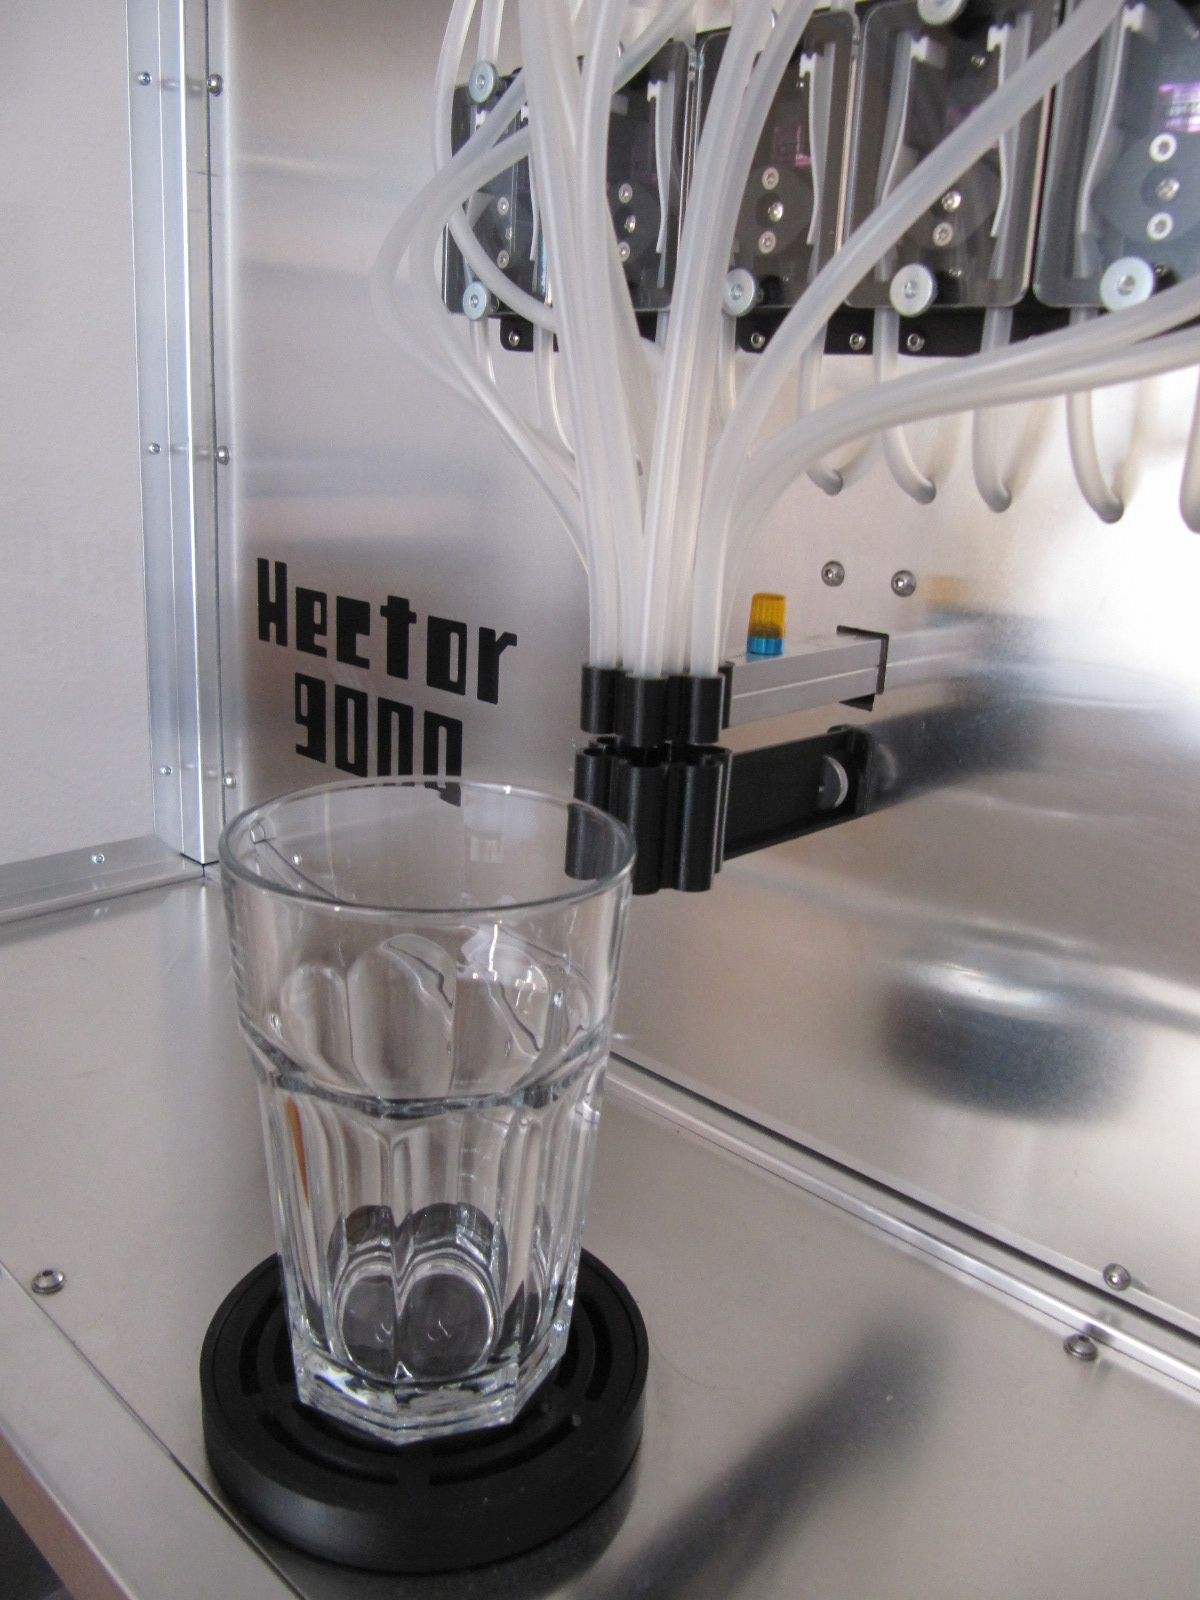
\includegraphics[height=8cm]{pics/scale_glass.JPG}
  \caption{Scale with glass} \label{scale_glass}
\end{figure}

\begin{figure}
  \centering
  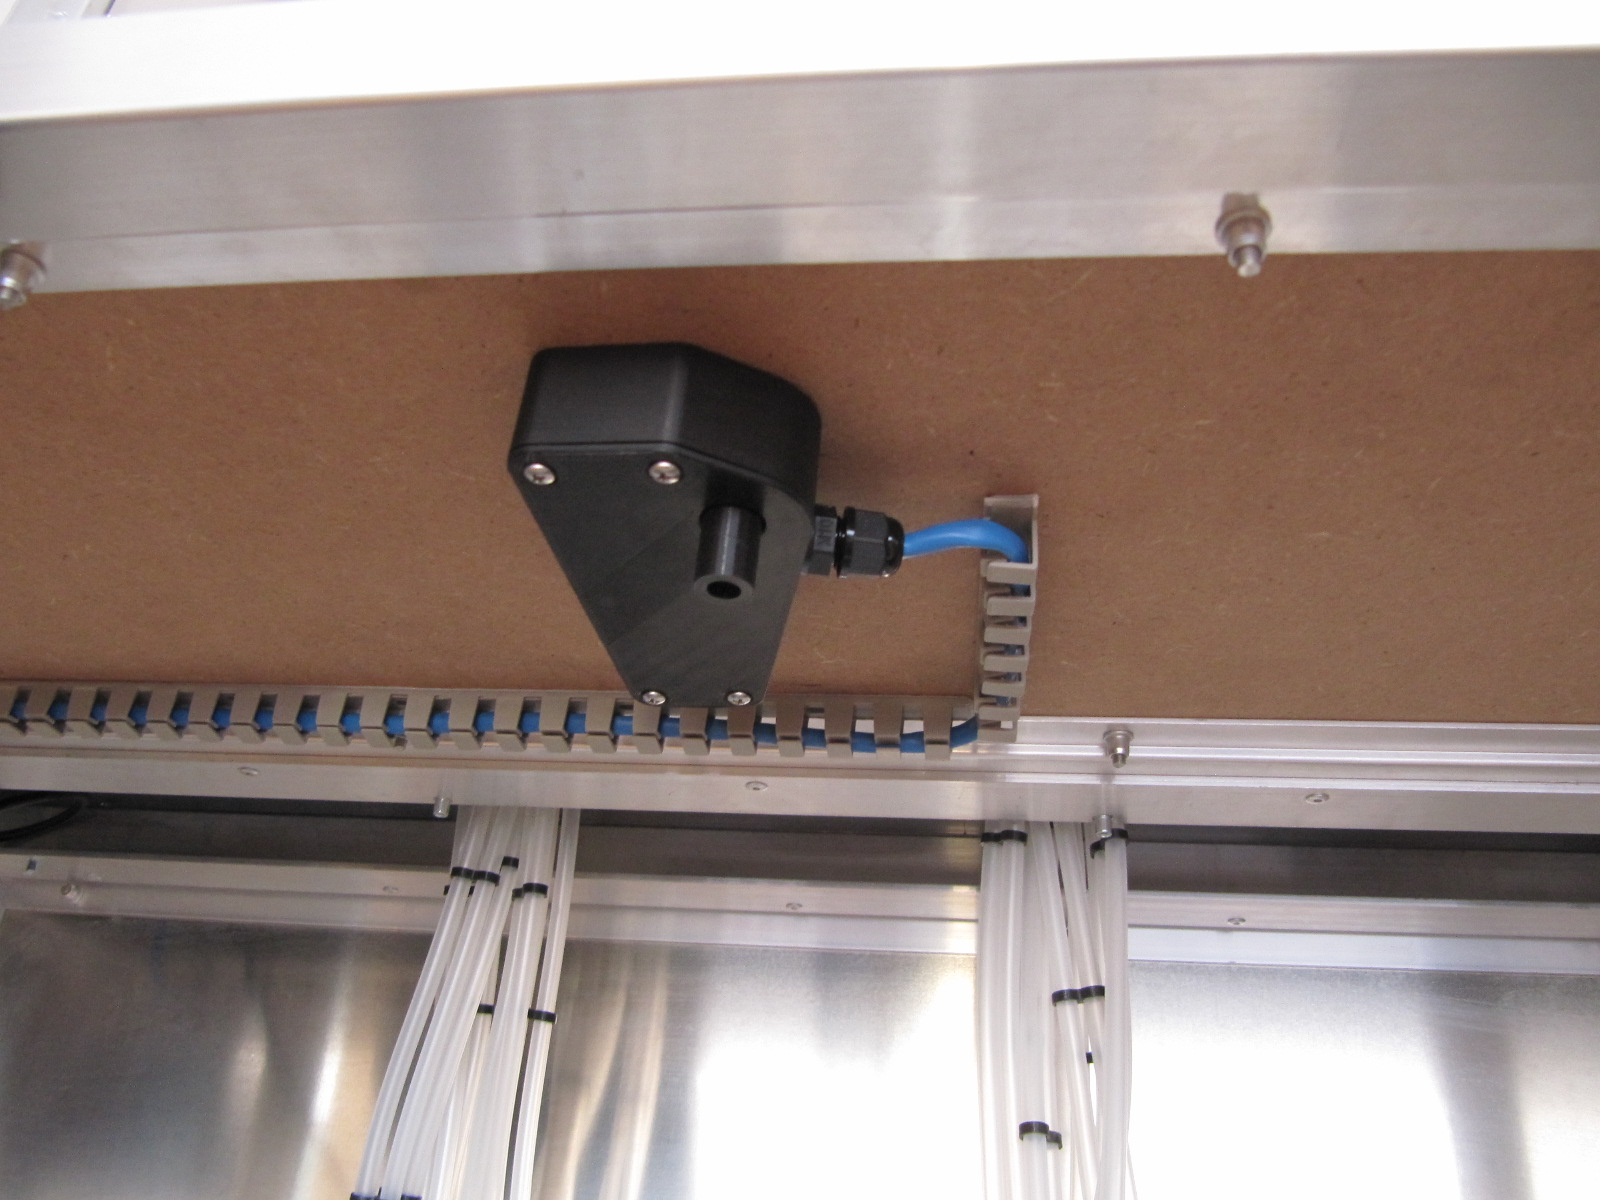
\includegraphics[height=8cm]{pics/scale_bottom.JPG}
  \caption{Bottom of the scale}
\end{figure}
  
\subsubsection{Pump}
To create the overpressure in the bottles, we use an air pump for fish tanks. Since the complete electronics operate with max.~12\,VDC, we opted for a 12\,V pump from Schego. The selection of the pump is relatively uncritical since the required pressure and the flow rate are low. It should only be ensured that the pump works oil-free. Because the pump has only one hole for mounting, a bracket has been designed. The following sequence during assembly has proven itself:

\begin {enumerate}
  \item Screw on 2 nuts at each end of the threaded rods and counter. A nut should be flush with the threaded rod, the key surfaces of the nuts must be in alignment.
  \item Insert threaded rods in the holes of the bracket,
  \item Screw the bracket into the housing,
  \item Insert pump and clamp with the U-profiles (optionally with foam rubber strips under the U-profiles),
  \item Counter the nuts (or glue with Loctite).
\end{enumerate}

\begin{figure}
  \centering
  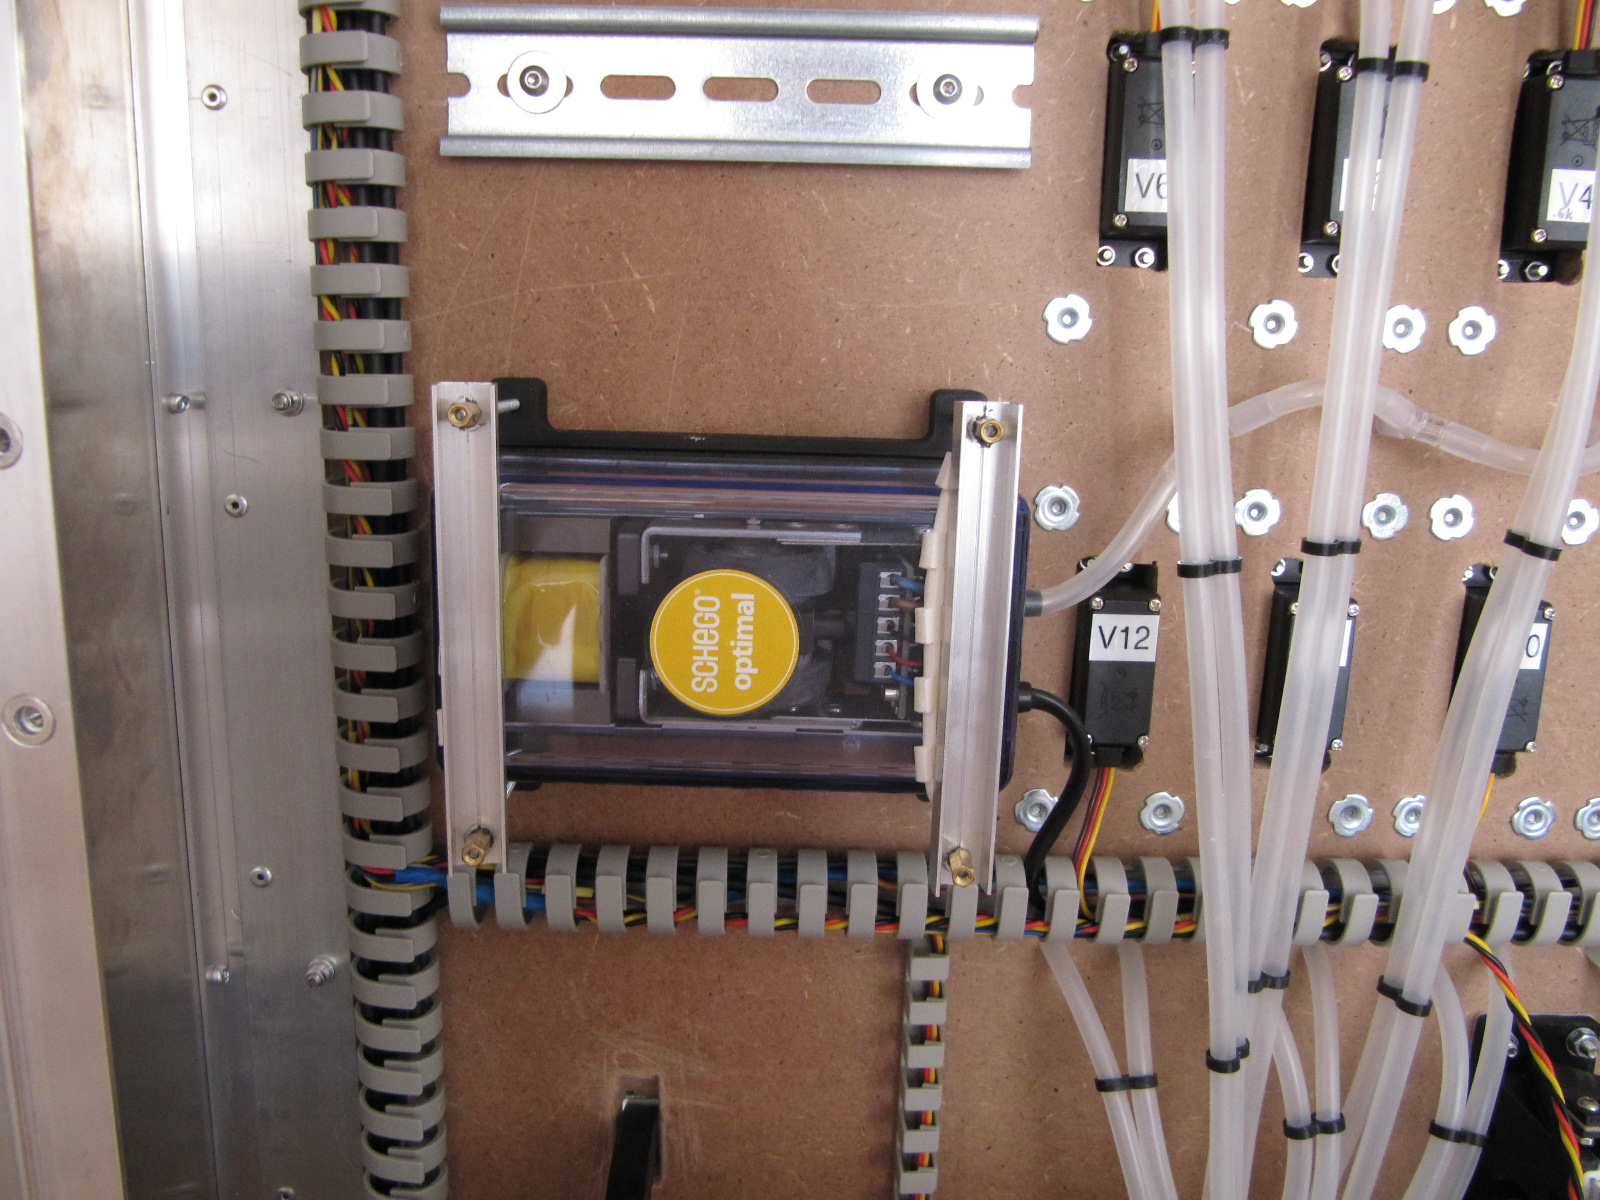
\includegraphics[height=8cm]{pics/pump.JPG}
  \caption{Airpump} \label{pump}
\end{figure}
\newpage

\subsubsection{Valves}
In order to realize the dosing of the fluids, pinch valves were designed for our cocktail machine which simultaneously open and close both hoses (i.\,e.~air and liquid) for an ingredient. \\
The required plastic parts for the valves can be printed without support. The (optional) cover was cut out of transparent PMMA with a CO\textsubscript{2} laser. Make sure the servos are original \textit{TowerPro MG996R}.  There are servos with the same name of no-name vendors. These servos may differ in the outer dimensions, in some cases significantly different from the original servos.  The round servo arms supplied with the servos must be adapted to the inner diameter of the cams. Special care is necessary: If the servo arms are eccentric in the cam, the valve will not close properly. Our servo arms were machined on a CNC milling machine with a very sharp wood 
cutter. The mounting holes for the servo arms are best drilled using the cam as a template. The screws for connecting cam and servo arm are secured with Loctite. Make sure the tongues are made of a material with good sliding properties. Our tongues were printed from \textit{Iglidur I150}. The tongues in the valves of Uncle Hector have been through a few hundred cycles and still work flawlessly. Alternatively, the tongues could be printed from PET, but this has not been tested yet. For the valves to sit flush with the rear wall, cutouts for the servos must be made (Fig.\,\ref{valve_rear}). For fastening the valves, captive nuts have been proven.

\begin{figure}
  \centering
  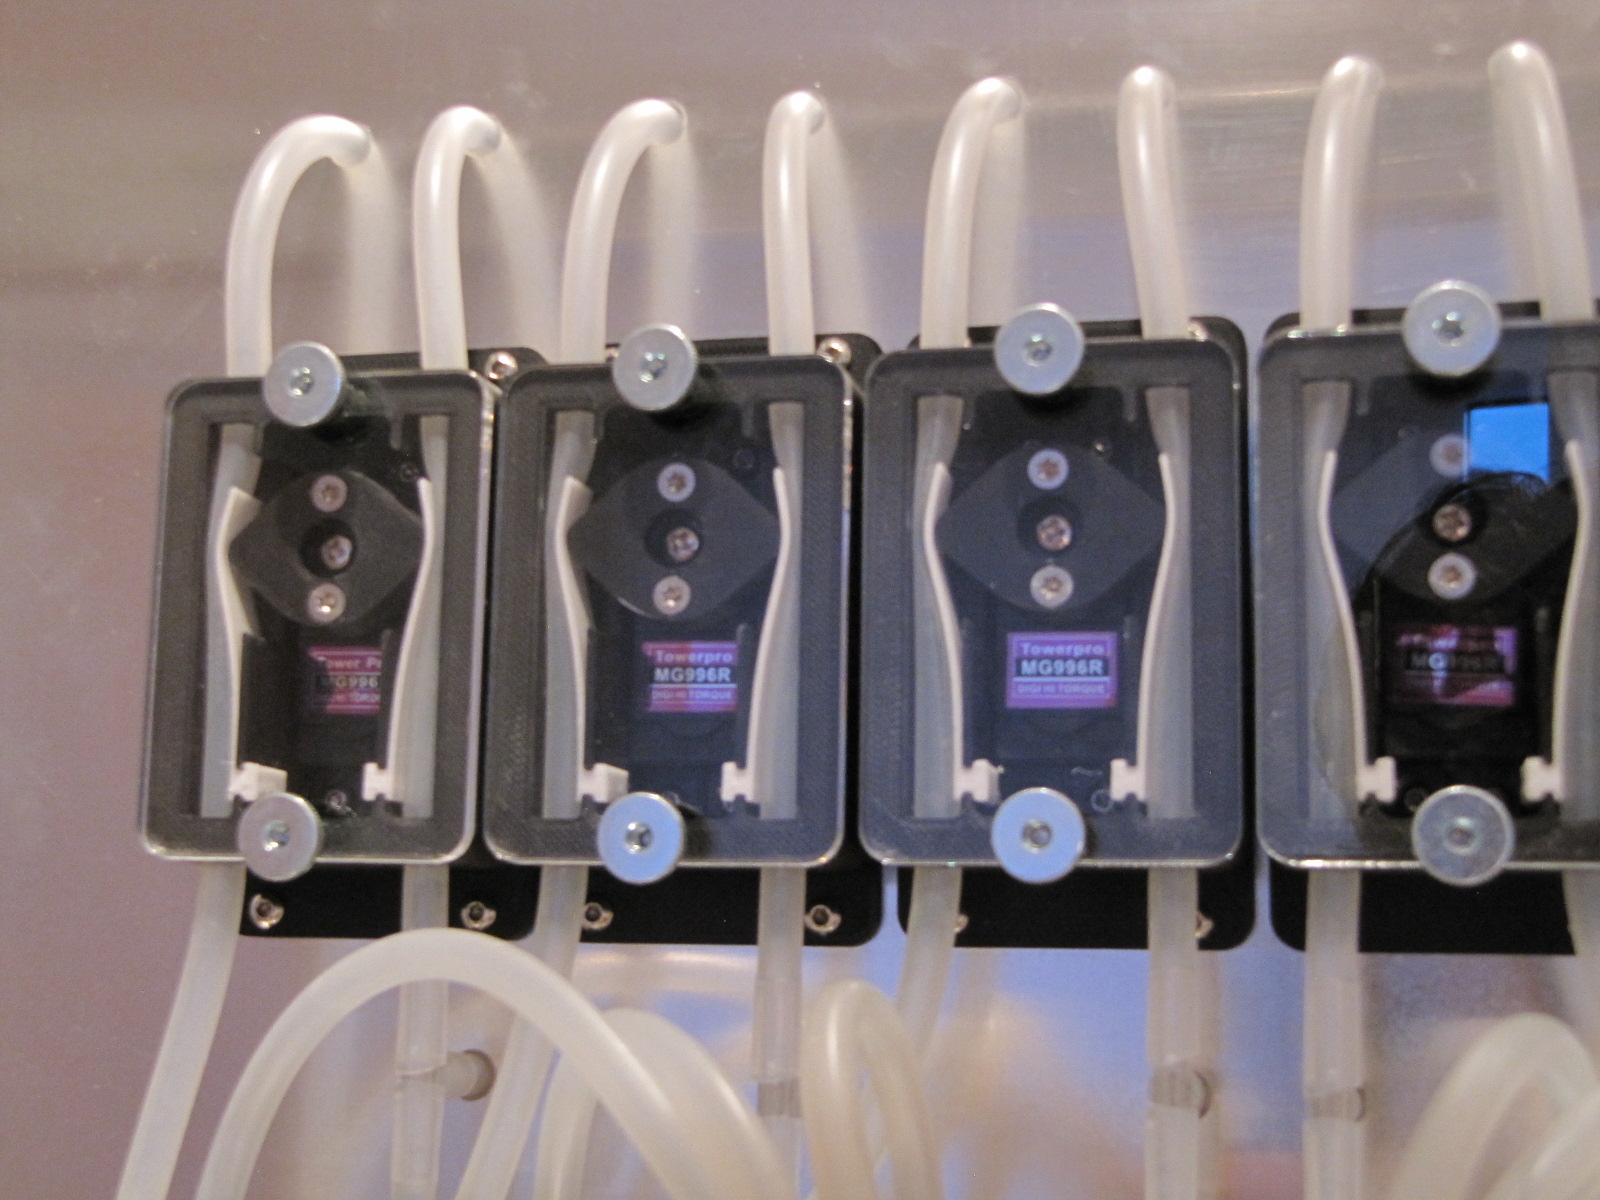
\includegraphics[height=8cm]{pics/valve_front}
  \caption{Valves} \label{valve_front}
\end{figure}

\begin{figure}
  \centering
  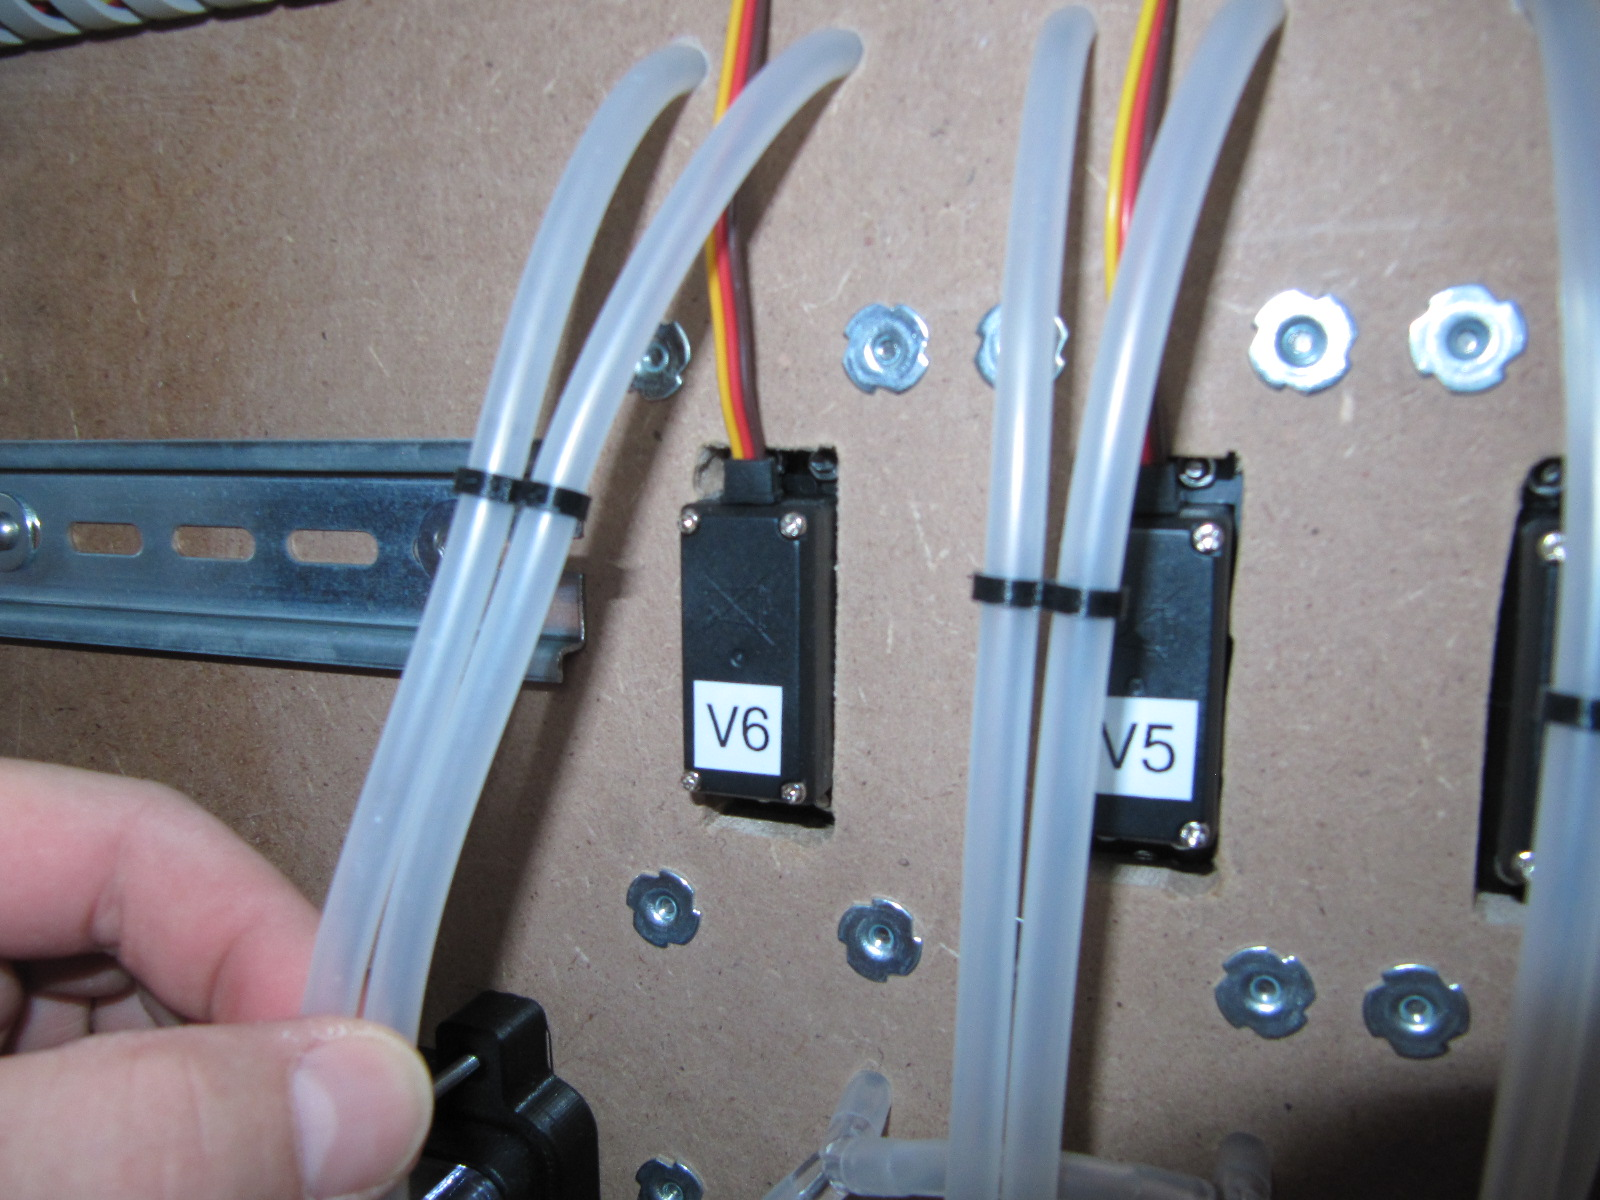
\includegraphics[height=8cm]{pics/valve_rear}
  \caption{Valves (rear view)} \label{valve_rear}
\end{figure}

\subsubsection{Arm}
In order to make the filling process more comfortable, the arm with the dosing head is retracted in the idle state (Fig.\,\ref{arm_front_in}). When the dosing process is started, the arm moves forward. All required plastic parts can be printed without support. The gliding insert should be made of a material with good sliding properties. Our gliding insert was printed from \textit{Iglidur I150}. Alternatively, the slide insert could be printed from PET, but this has not been tested yet. The boom consists of an aluminum profile with \SI{15.5}{\milli\metre} edge length. Such profiles can be found in almost every German DIY store. The pinion is pressed onto the shaft of the motor and needs no further securing. To attach the rack to the boom, M3 blind rivet nuts were inserted into the profile. The dosing head is secured with a self-tapping screw in the profile. The trigger is glued to the boom. The trigger has a hole through which a cable was routed to power an optional all-round light on the arm. \\
When mounting the arm, make sure that the bottom bolt is passed through the hole from the rear and screwed down with a regular nut. The upper bolts are inserted from the front through the rear wall. The drip catcher can now be mounted on the lower screw with a knurled nut (Fig.\,\ref{drip}). 

\begin{figure}[H]
  \centering
  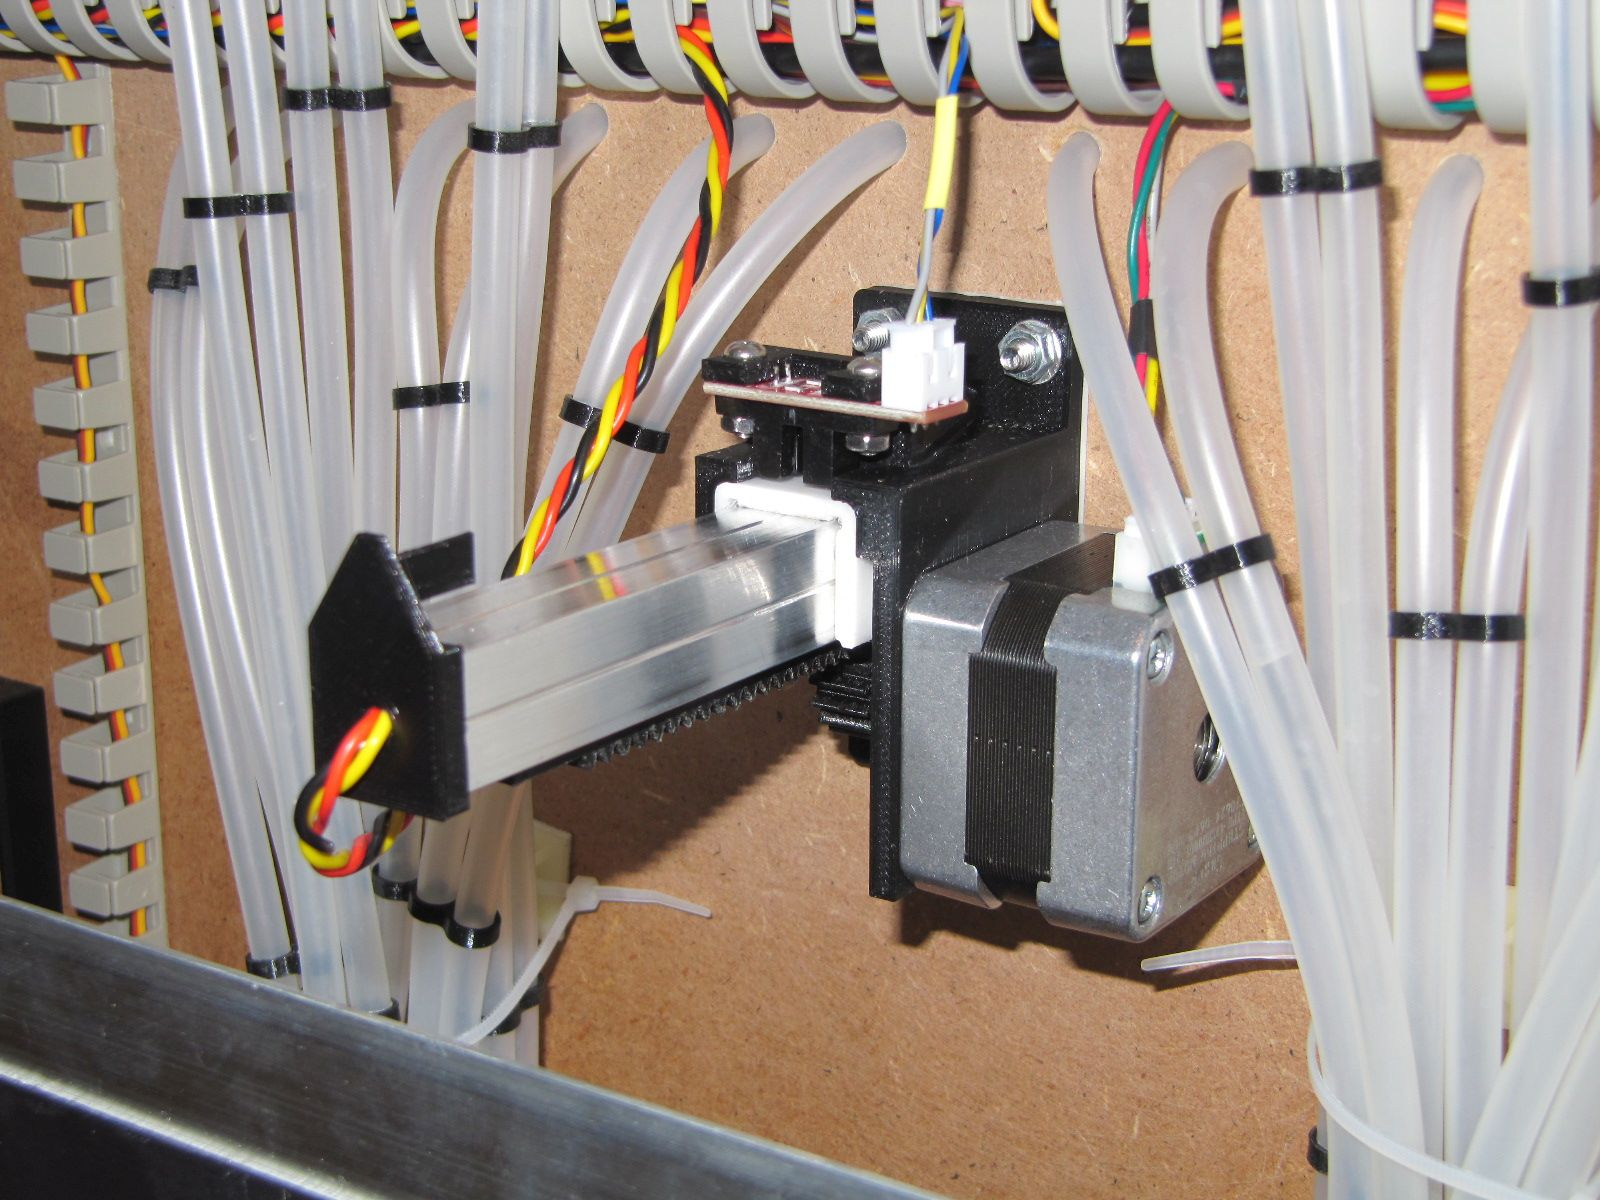
\includegraphics[height=8cm]{pics/arm_rear.jpg}
  \caption{Arm (rear view)} \label{arm_rear}
\end{figure}

\begin{figure}
 \centering
 \subfigure[Arm retracted]{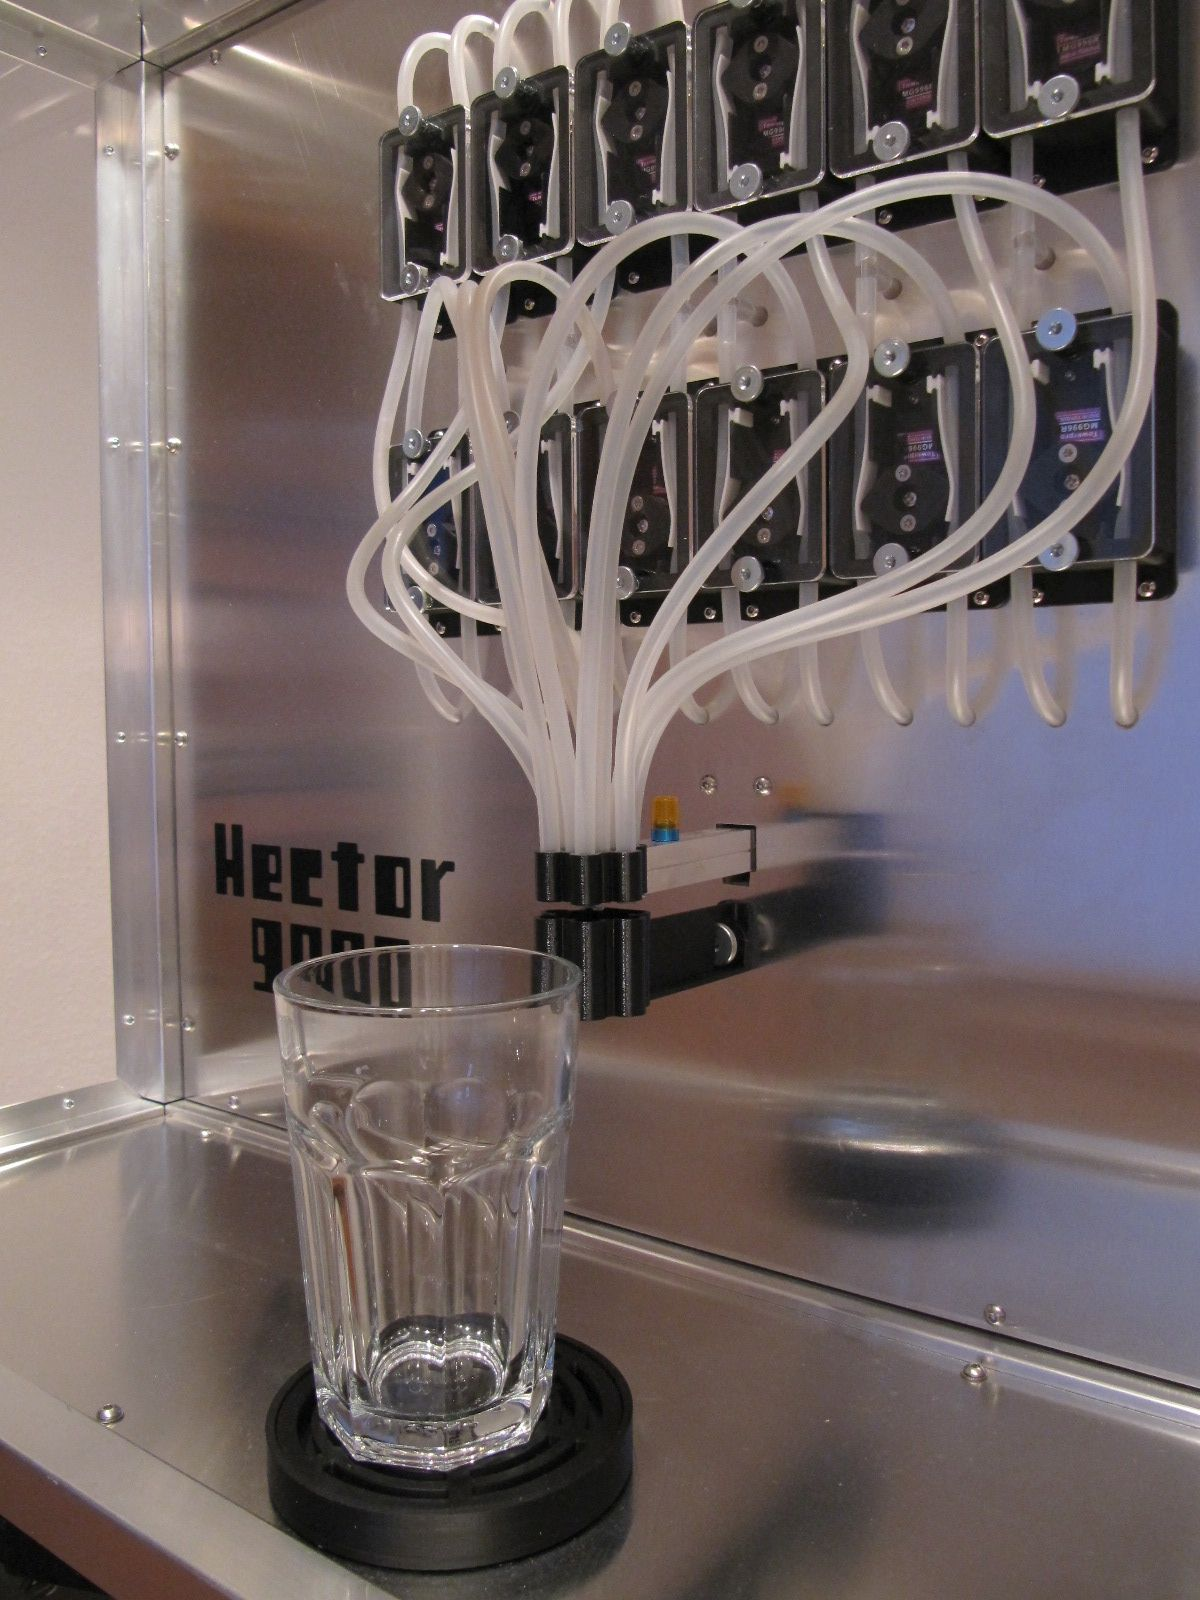
\includegraphics[height=8cm]{pics/arm_front_in.jpg}}
 \subfigure[Arm moved forward]{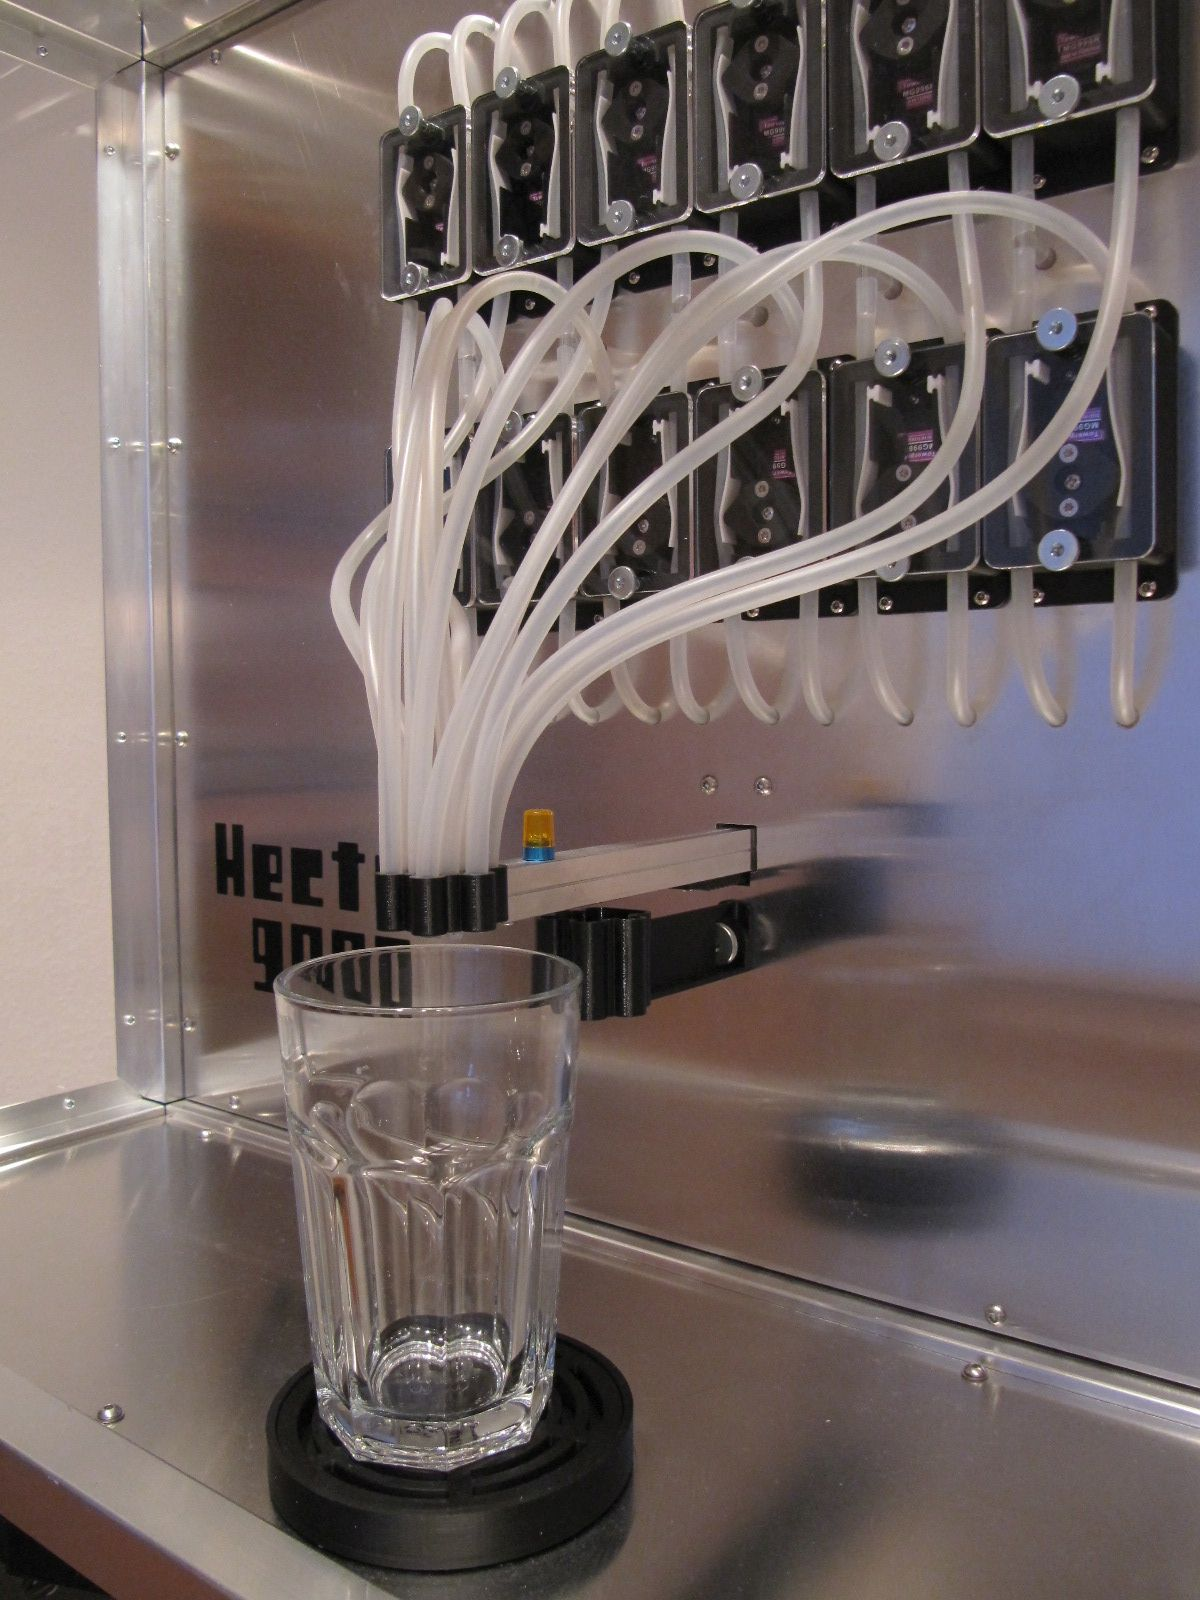
\includegraphics[height=8cm]{pics/arm_front_out.jpg}}
 \caption{Endpositions of the arm} \label{arm_front_in}
\end{figure}

\begin{figure}
  \centering
  \subfigure{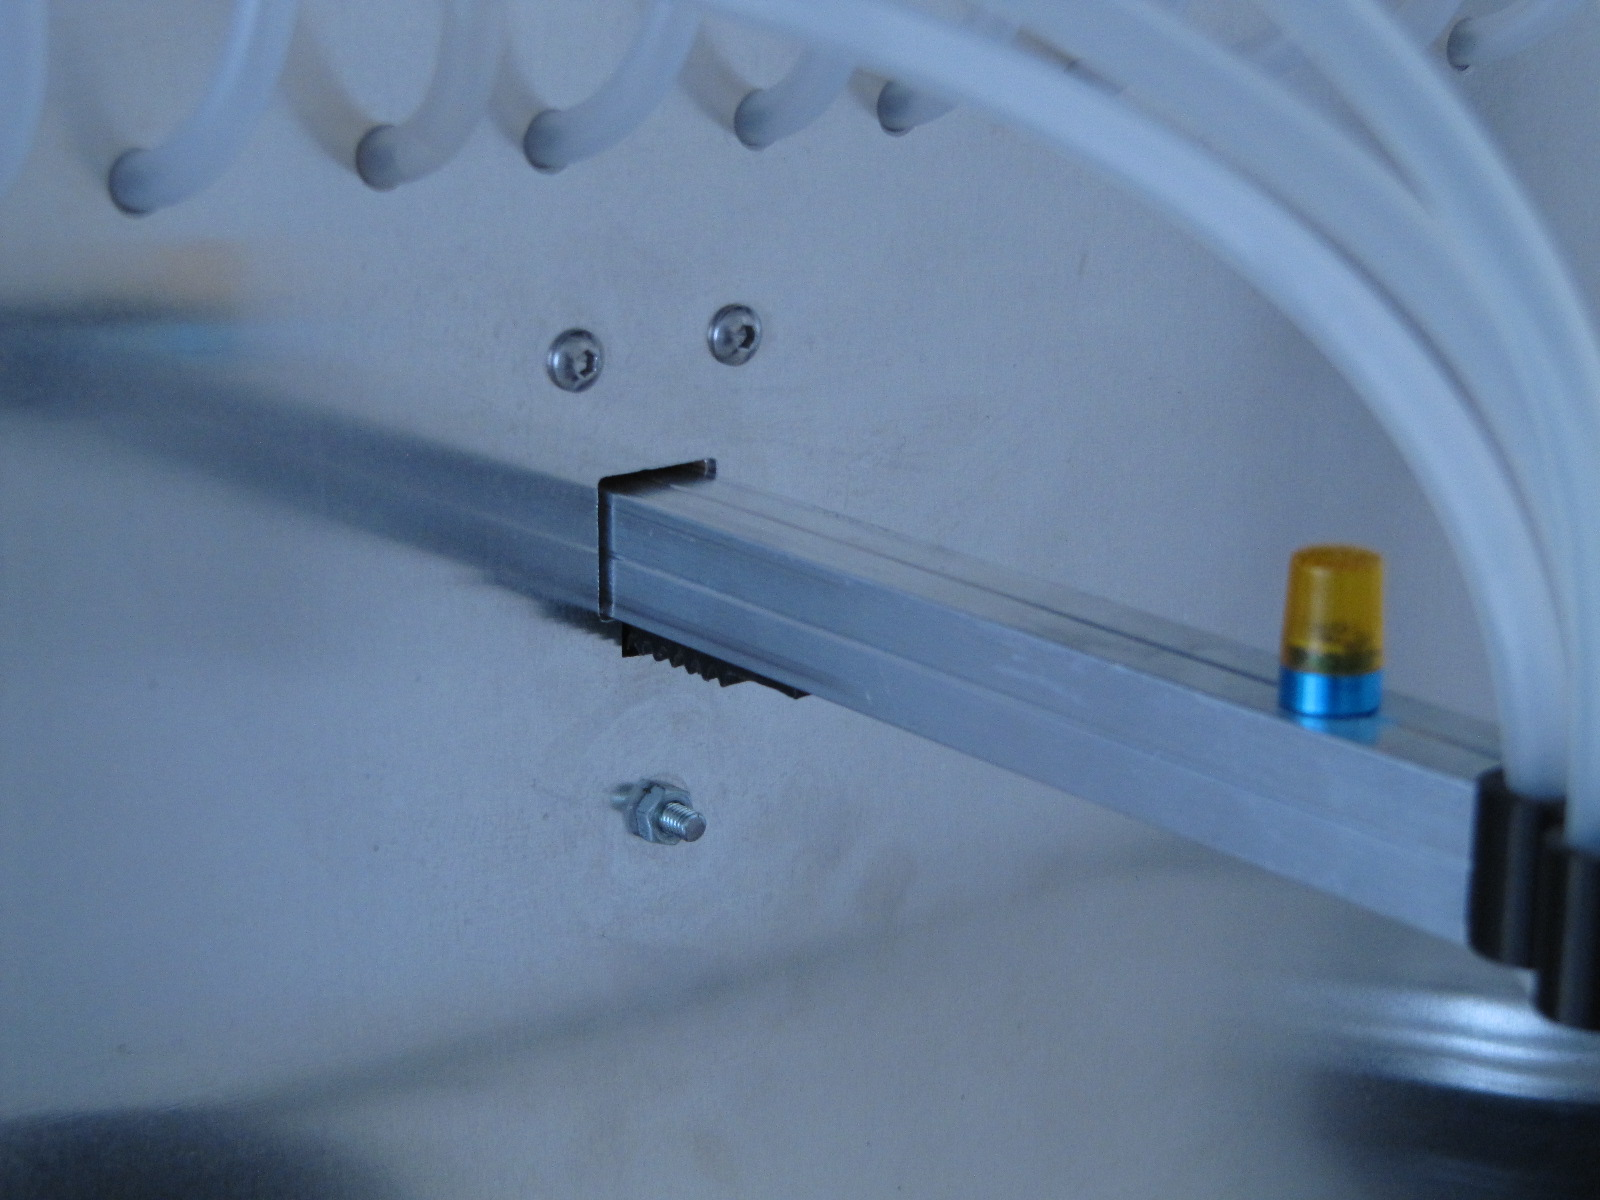
\includegraphics[height=8cm]{pics/nodrip.jpg}}
  \subfigure{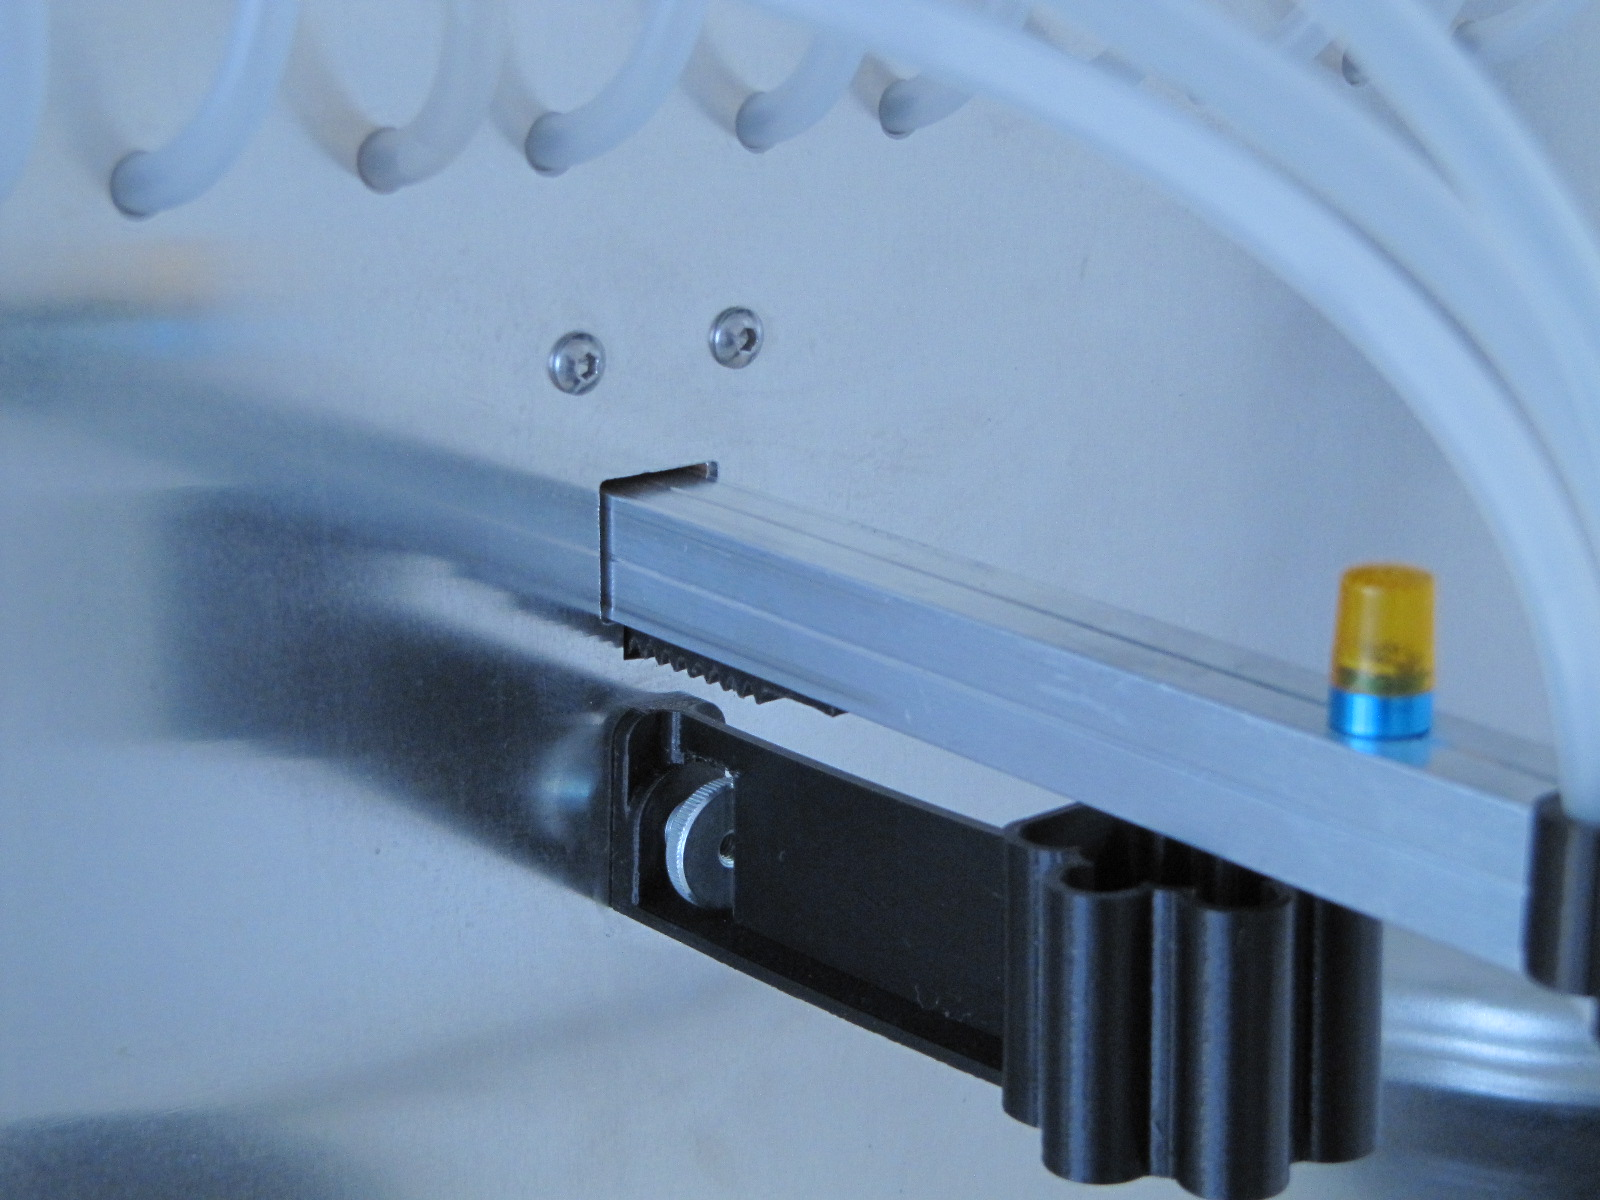
\includegraphics[height=8cm]{pics/yodrip.jpg}}
  \caption{Mounting of the drip catcher} \label{drip}
\end{figure}

\subsubsection{Bell}
When building the mechanism for the bell, make sure that the center of the bell is \SI{100}{\milli\metre} away from the rotational axis of the arm. A bracket is provided for attaching the bell (Fig.\,\ref{bell_mount}). To drill the necessary holes in the bell, the bracket is used as a drilling jig. The mounting of the finger on the back wall is actually self-explanatory. To attach the motor bracket (Bell\_servo-bracket.stl) to the rear panel, it is advisable to use captive nuts or threaded inserts, so the finger can be easily adjusted later (Fig.\,\ref{finger}).

\begin{figure}
  \centering
  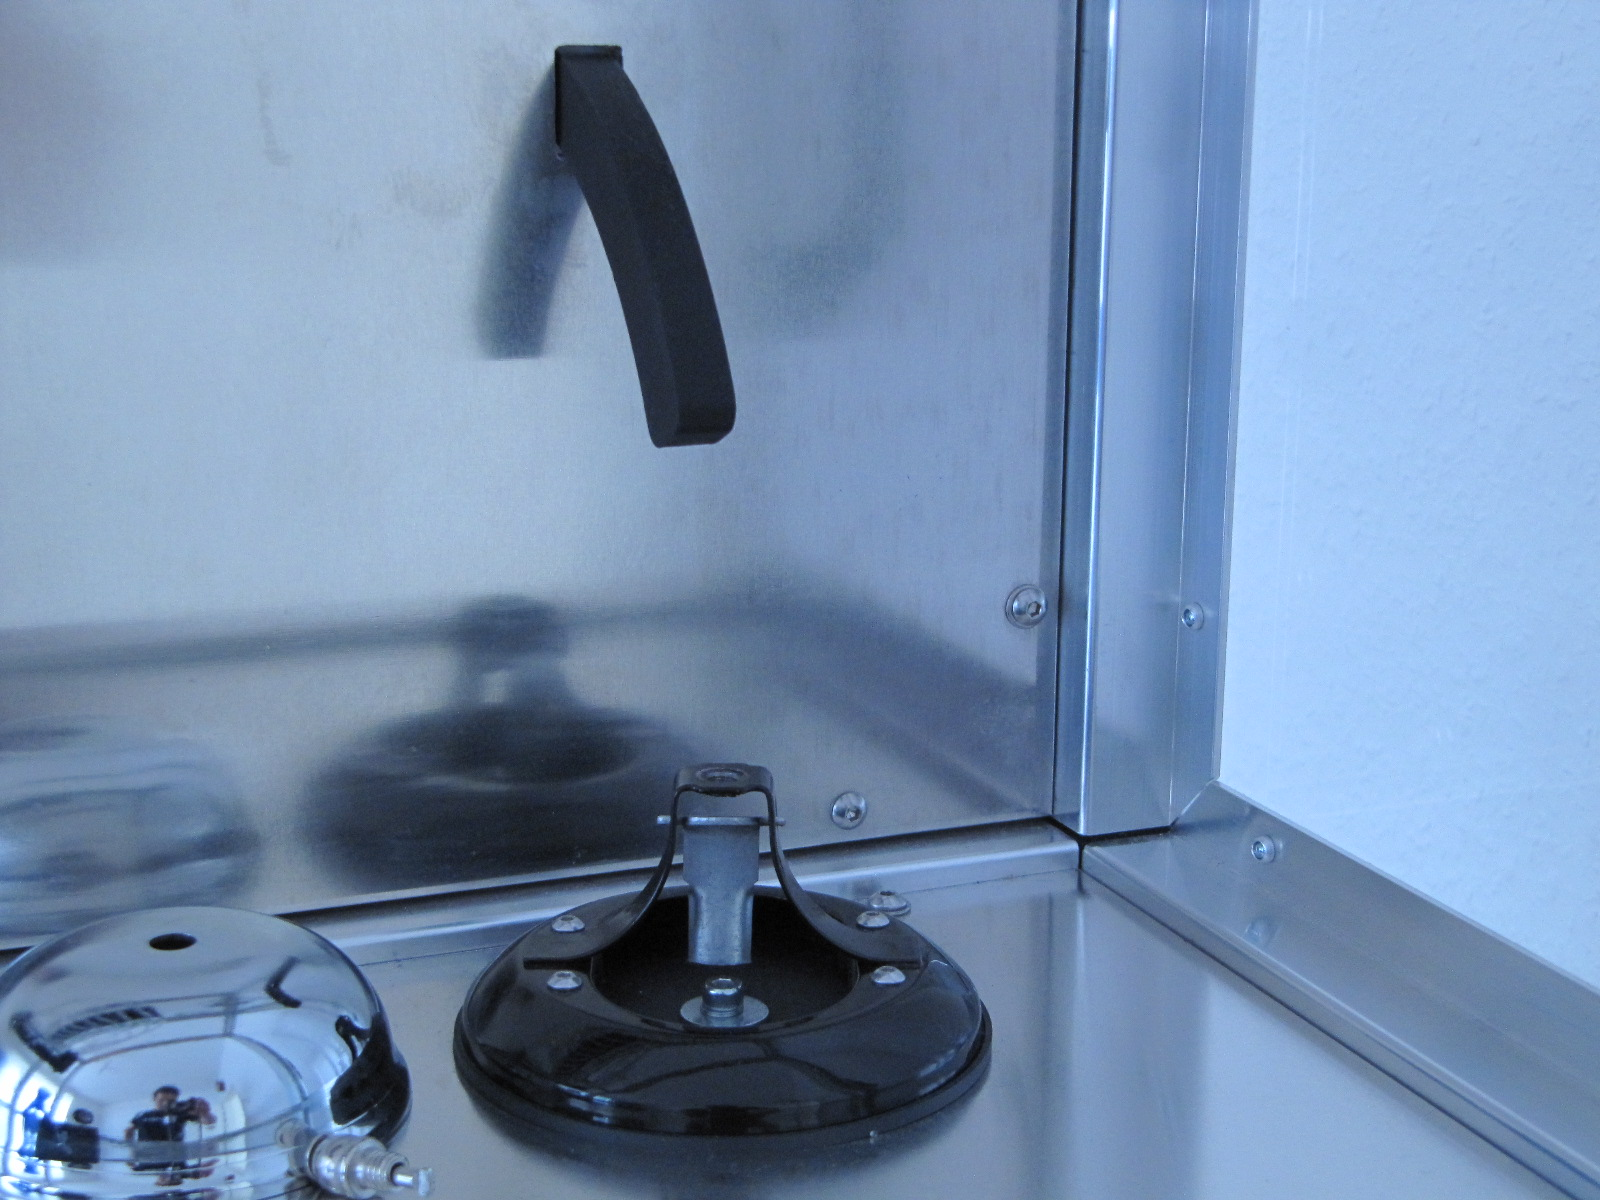
\includegraphics[height=8cm]{pics/bell_mount.JPG}
  \caption{Mounting of the bell} \label{bell_mount}
\end{figure}

\begin{figure}
  \centering
  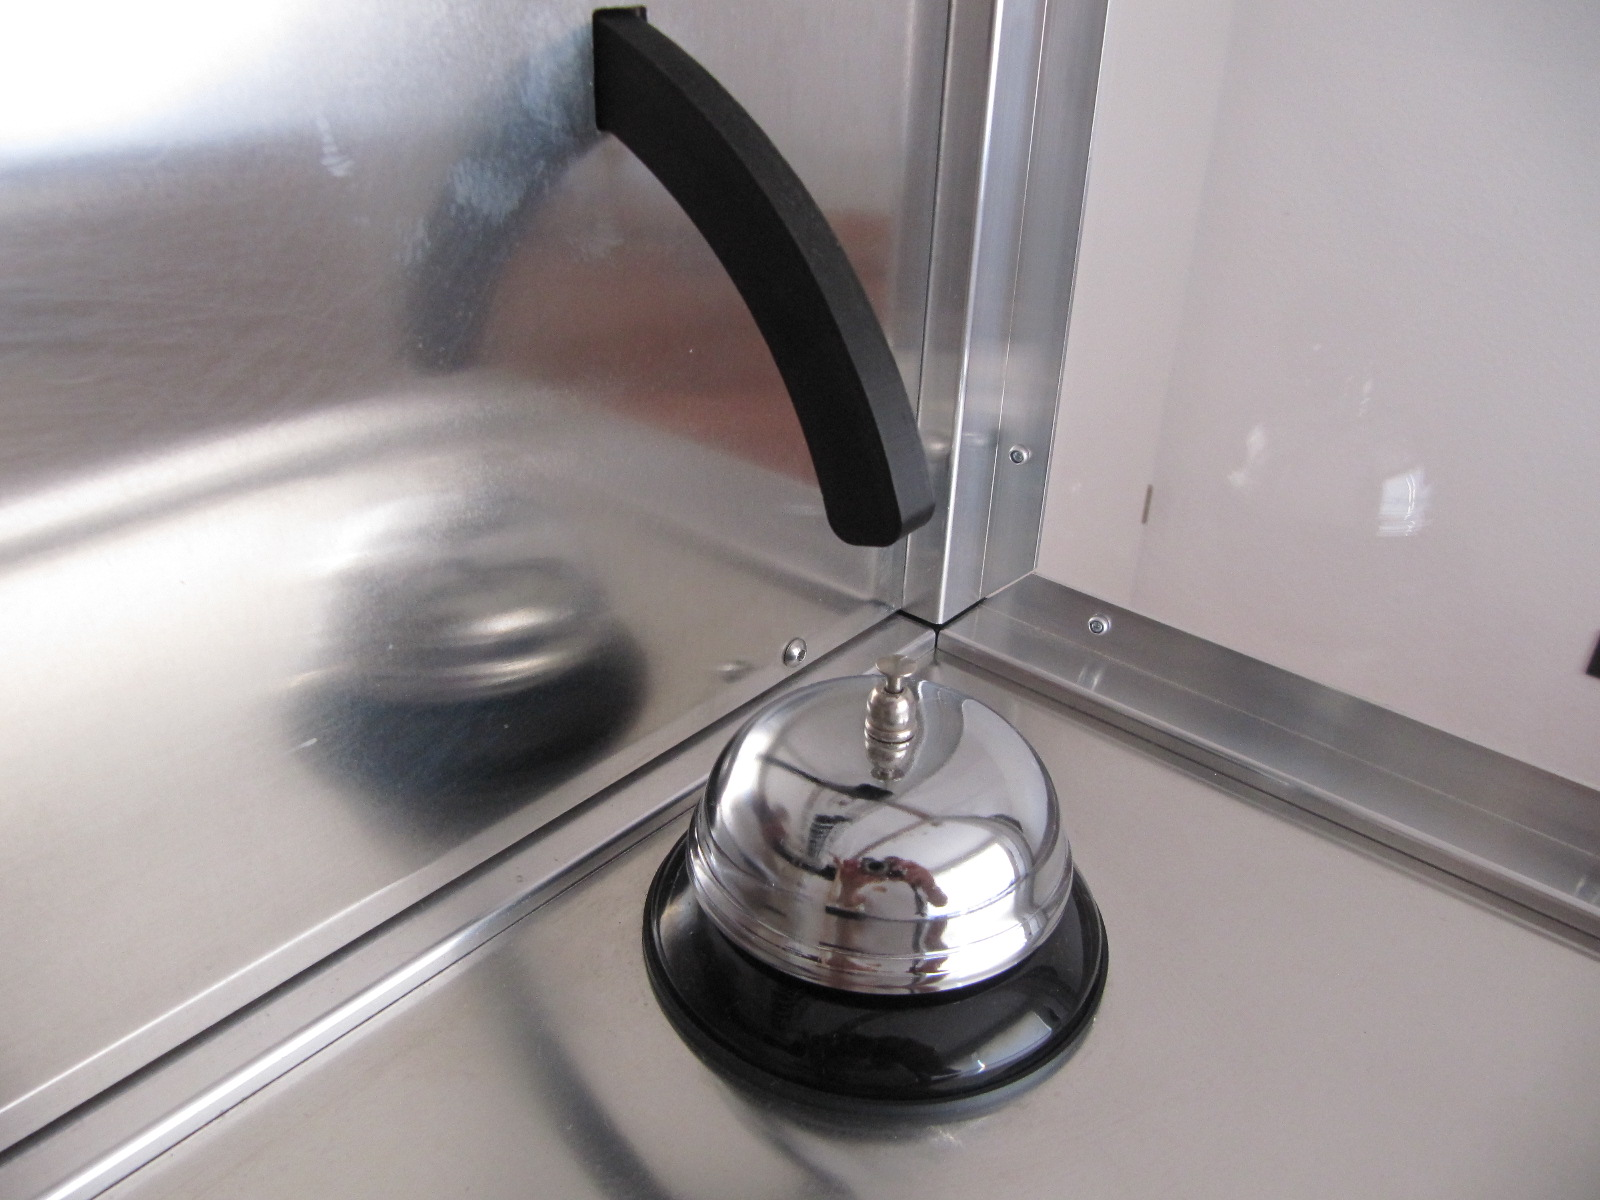
\includegraphics[height=8cm]{pics/bell.JPG}
  \caption{Bell} \label{bell}
\end{figure}

\begin{figure}
  \centering
  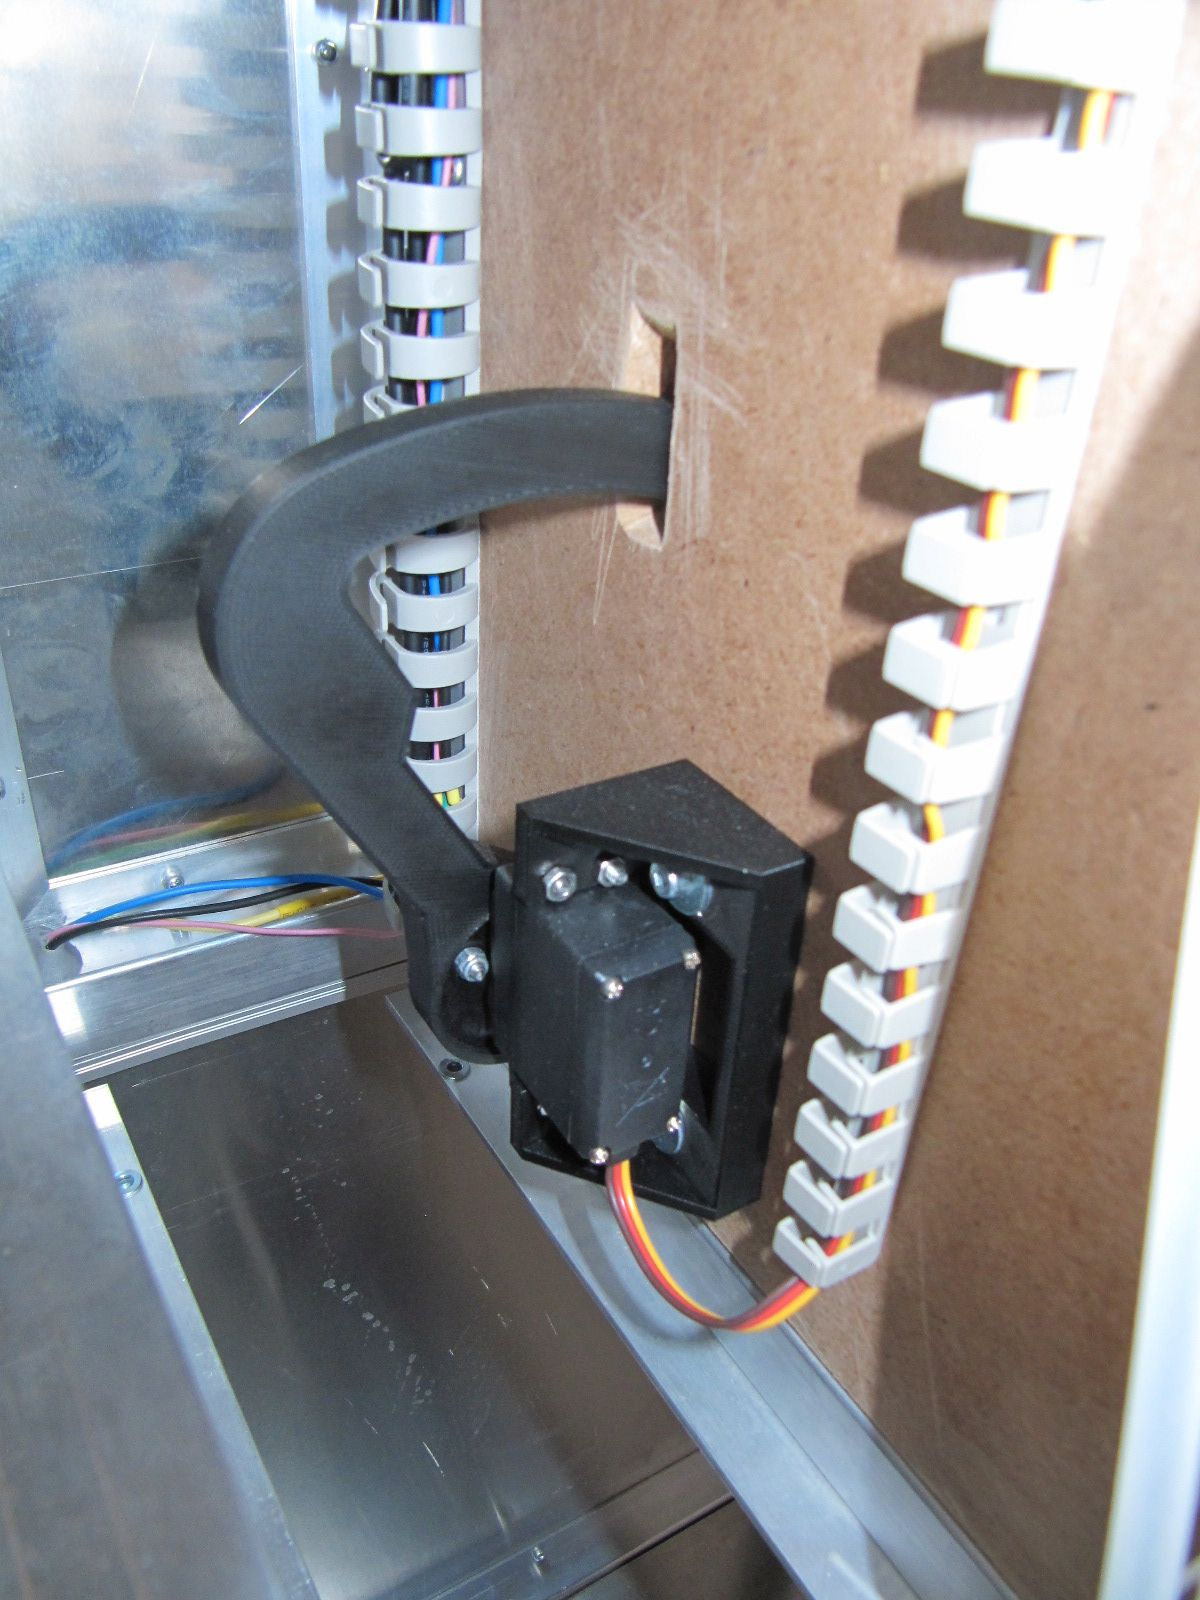
\includegraphics[height=8cm]{pics/finger.JPG}
  \caption{Finger with bracket} \label{finger}
\end{figure}

\subsubsection{Hoses}
To transport liquids and air, silicone hoses with an outer diameter of \SI {6}{\milli\metre} and \SI{4}{\milli\metre} inside diameter are used. In any case, care must be taken that the hoses are intended for use with food. To guide the hoses through the housing, the valves and the dosing head, it has been proven to cut off one end at an acute angle.
For each ingredient, two hoses are passed through a valve. One hose directs the liquids from the bottle to the dosing head, the other hose connects the air pump and the bottle. When guiding the hoses through the housing, care must be taken that the hoses do not tangle with the arm. We just used cable ties (Fig.\,\ref{hoses}).

\begin{figure}
  \centering
  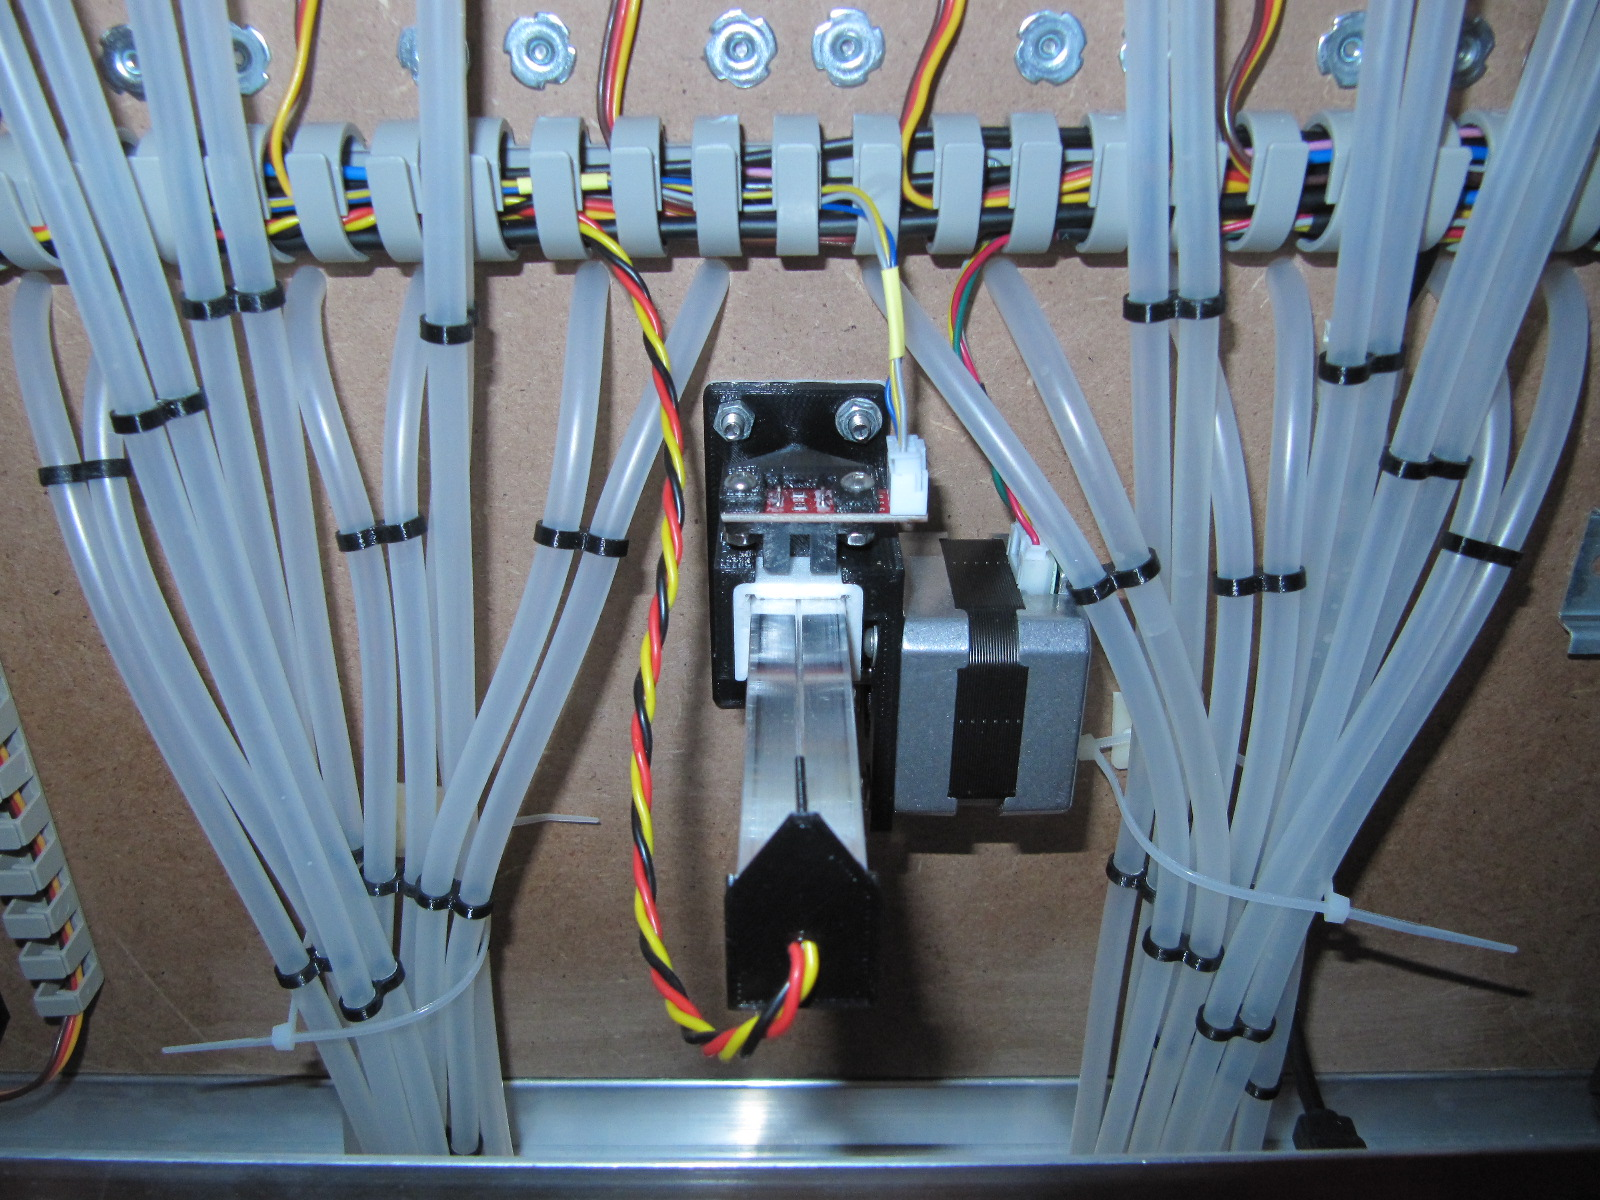
\includegraphics[height=8cm]{pics/hoses.JPG}
  \caption{Guiding the hoses} \label{hoses}
\end{figure}

\subsubsection{Plugs}
The plugs consist of a 3D printed core and a conical seal. The seal makes it possible to connect different beverage bottles with one kind of plug. The seals can be purchased from catering supplies. When printing the cores, food grade filament should be used. On one side of the plug are the hoses leading to the valves (do not confuse air and beverage hoses!) connected. On the other side of the plug is a piece of silicone tubing connected which reaches to the bottom of the bottle.

\begin{figure}
  \centering
  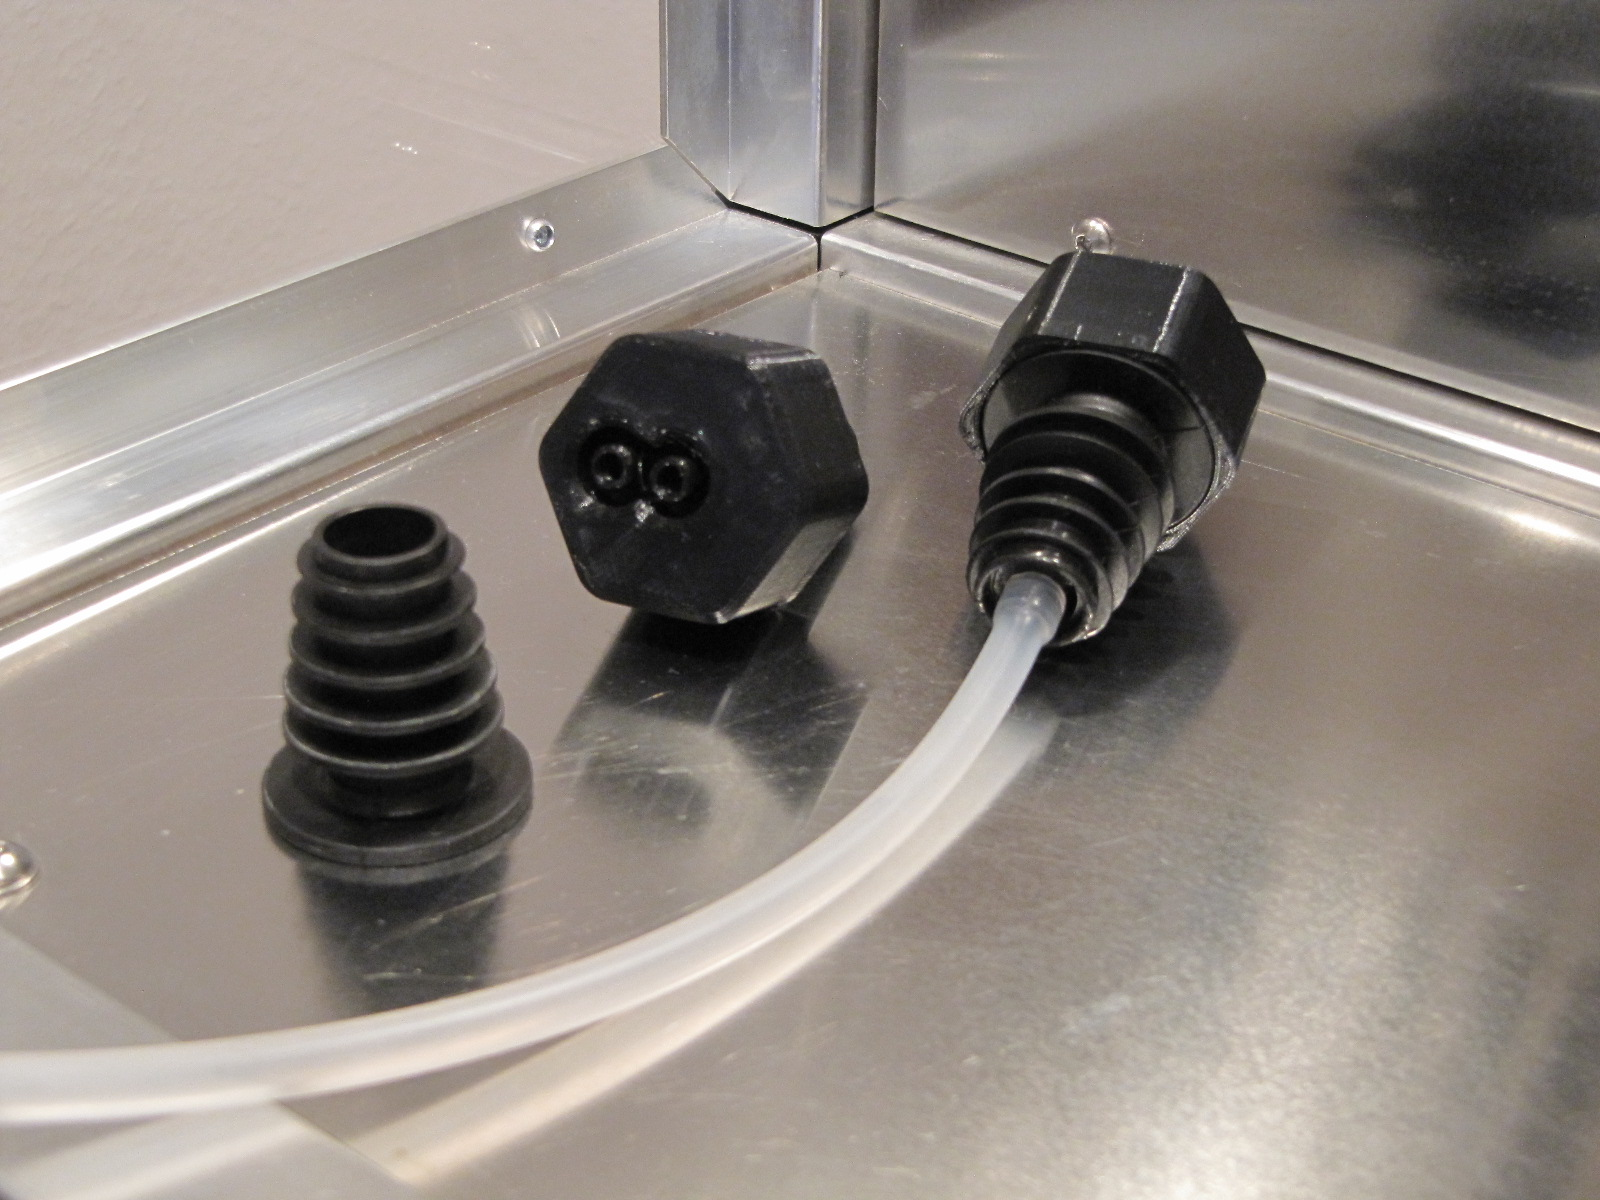
\includegraphics[height=8cm]{pics/plugs}
  \caption{Plugs} \label{plugs}
\end{figure}

\subsubsection{Flushing funnel}
As it takes a lot of water and time to rinse the hoses, it is not much fun to stand next to Hector and empty full glasses during the wash program. We have therefore constructed a flushing funnel that transports the wastewater directly into a bucket or spout. The flushing funnel can be printed without support. The hose nozzle is designed for a silicone hose with an internal diameter of \SI{10}{\milli\metre}.

\begin{figure}
  \centering
  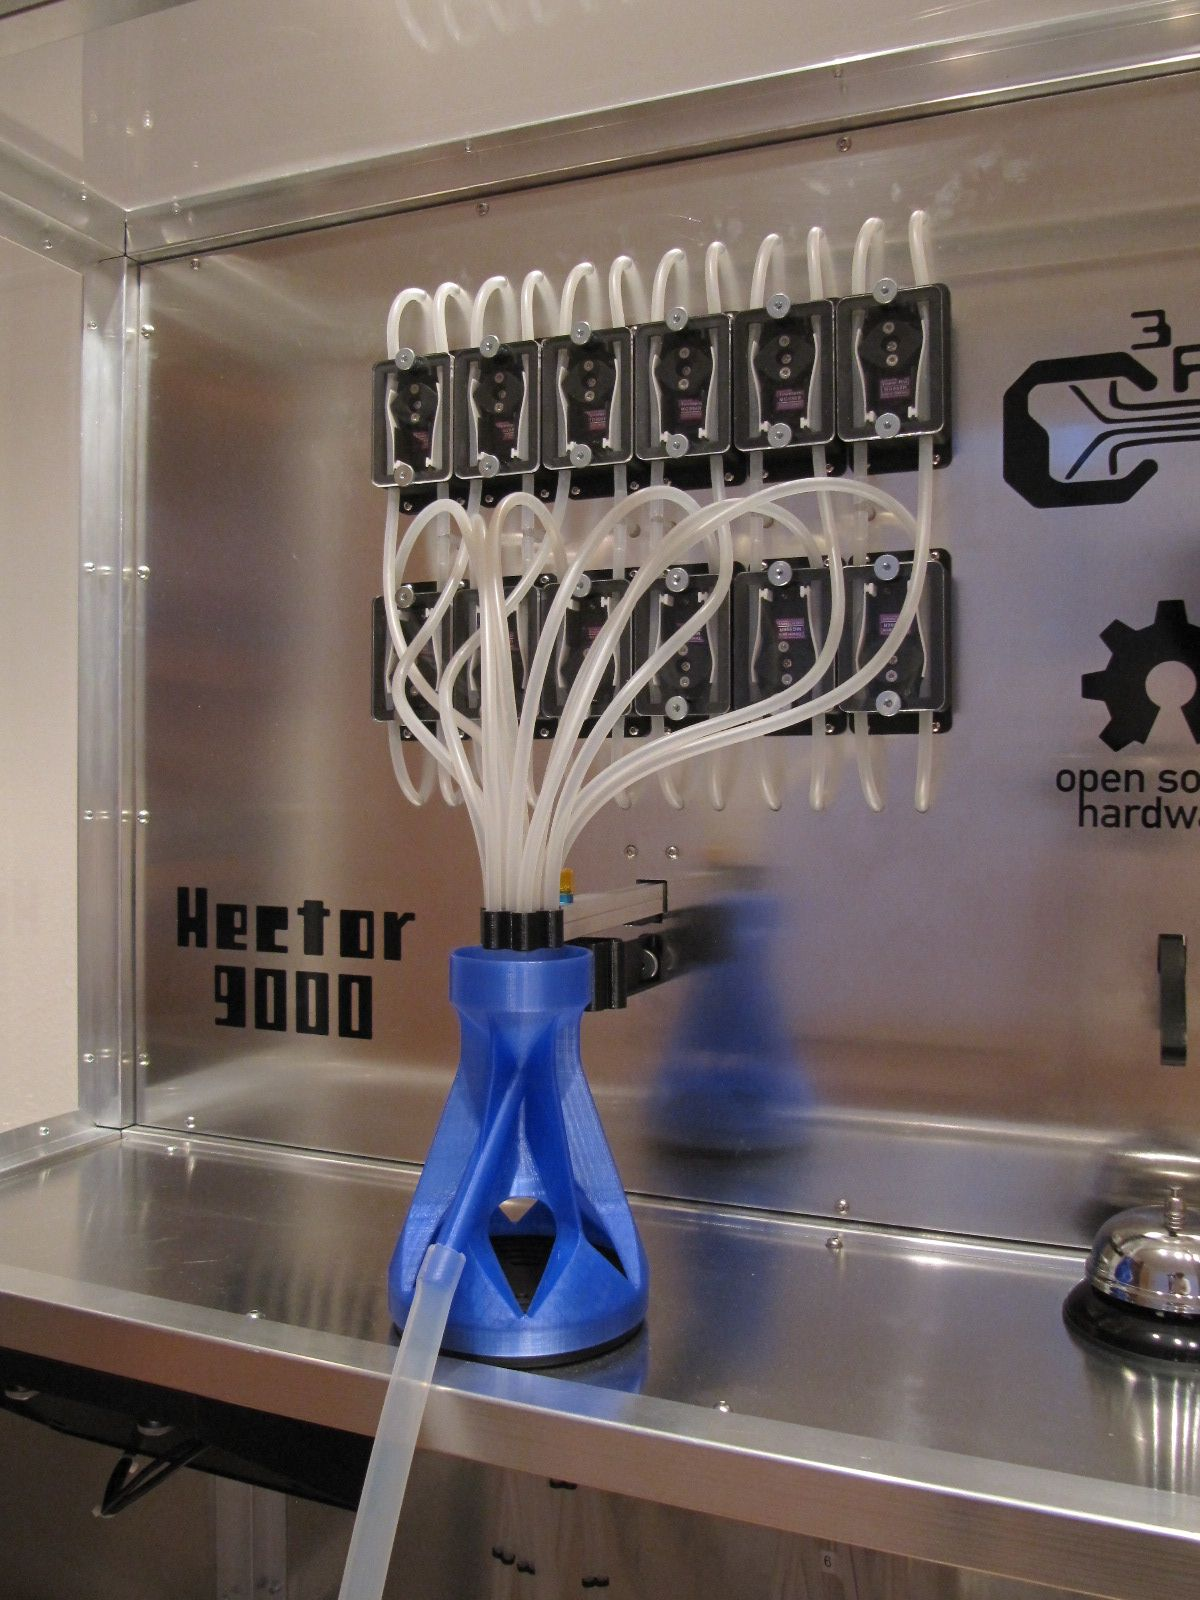
\includegraphics[height=8cm]{pics/funnel.JPG}
  \caption{Flushing funnel} \label{funnel}
\end{figure}

\subsubsection{Housing}
The housing consists of \SI{25}{\milli\metre} aluminum profiles that have been covered with aluminum sheets and PMMA sheets. The metal sheet on which the scale was attached, as well as the sheet metal which carries the valves, were additionally glued to an MDF board. Before bonding, captive nuts were placed into the MDF panels to later screw on the DIN rails and pump. The PMMA plates and most of the other plates were fixed with \SI{4}{\milli\metre} blind rivets. The rear wall is fixed by M4 screws. Blind rivet nuts were used in the profiles as a counterpart to the screws. It is strongly recommended to use special sheet metal drills for machining the sheets and profiles, otherwise problems may occur when inserting the rivets. The case is not included in the bill of materials, here everyone should let their creativity run free\footnote{Besides, we do not have complete CAD data for the case ;)}.

\begin{figure}
  \centering
  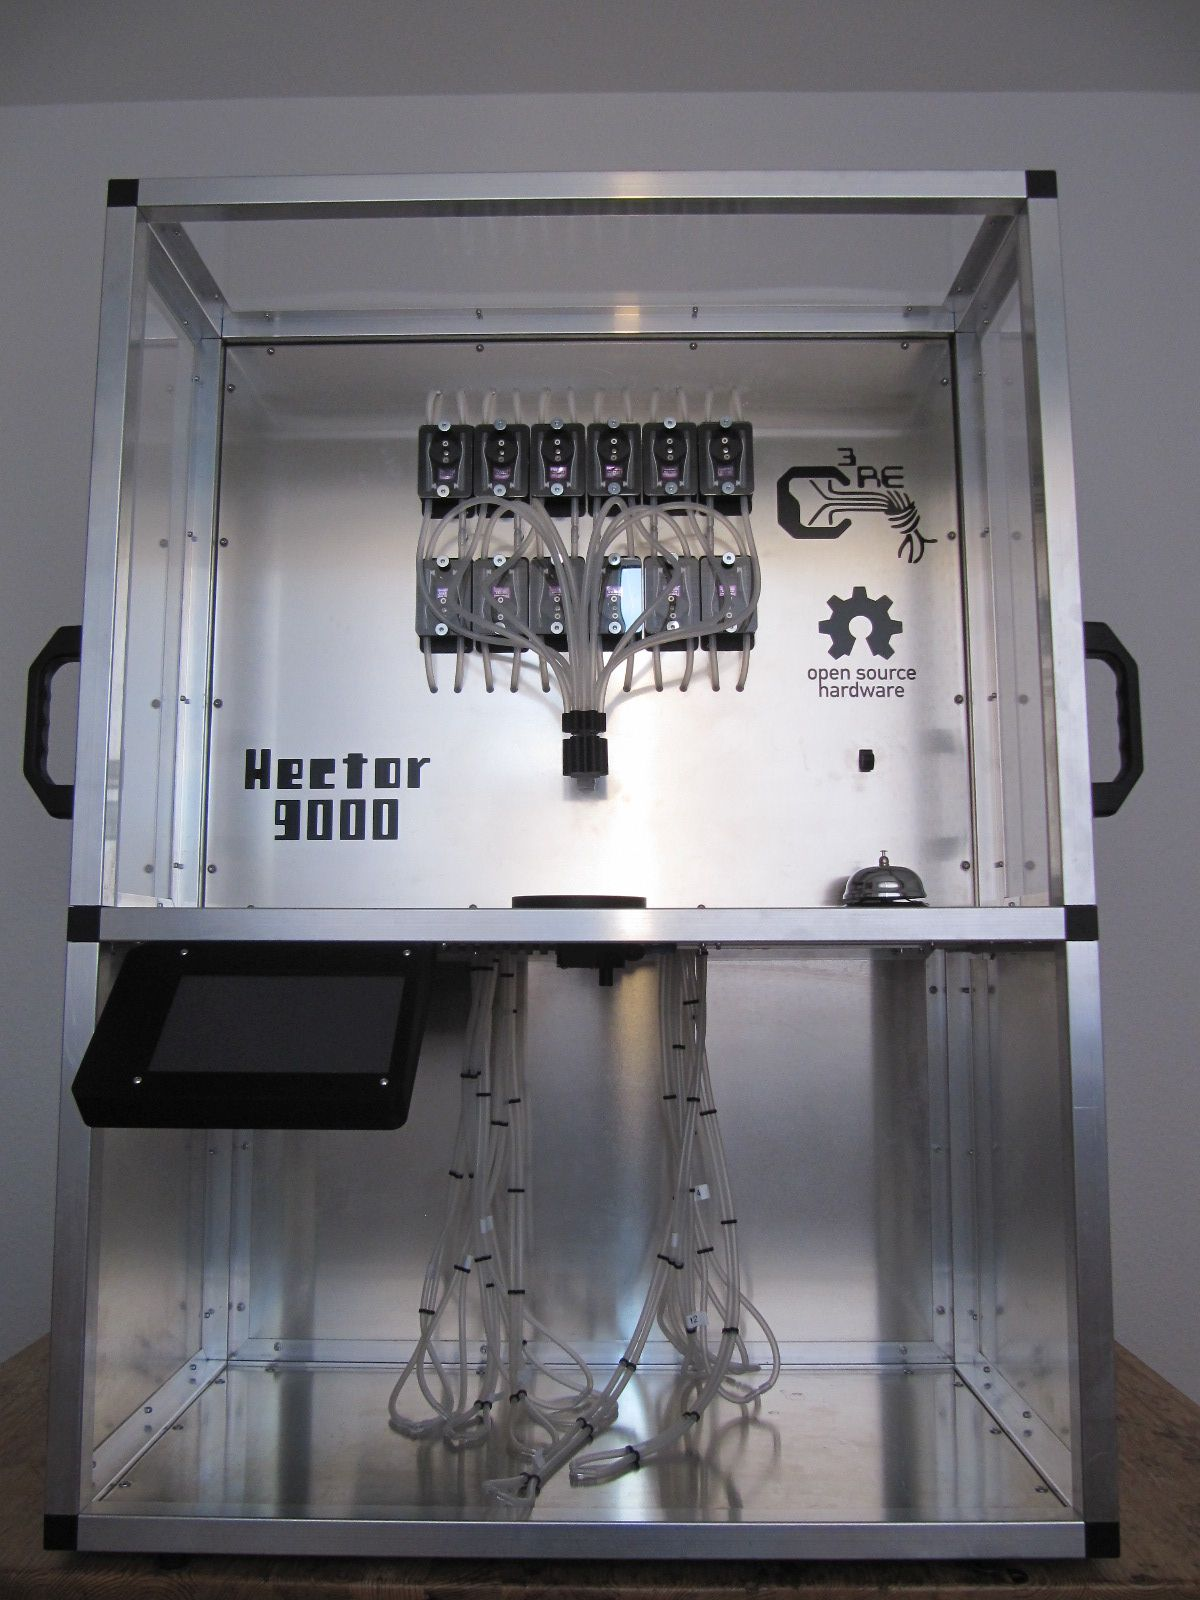
\includegraphics[height=8cm]{pics/hector9000.JPG}
  \caption{Hector 9000} \label{hector9000}
\end{figure}

\subsubsection{Display}
For the selection of drinks we have opted for a 7'' display with touch function via USB. The USB version is necessary because the GPIOs are used for other functions. The display is attached to a extruded profile of the housing. For transport the display can be turned into the housing (Fig.\,\ref{display_half_in}). In the printed housing for the display are 3 holes for mounting it to the frame. Only two holes are needed for the attachment: the middle hole and an outer one. The display is screwed to the frame by means of blind rivet nuts and knurled screws. To turn the display, remove the outer screw and loosen the center screw.


\begin{figure}
 \centering
 \subfigure[Display half flipped]{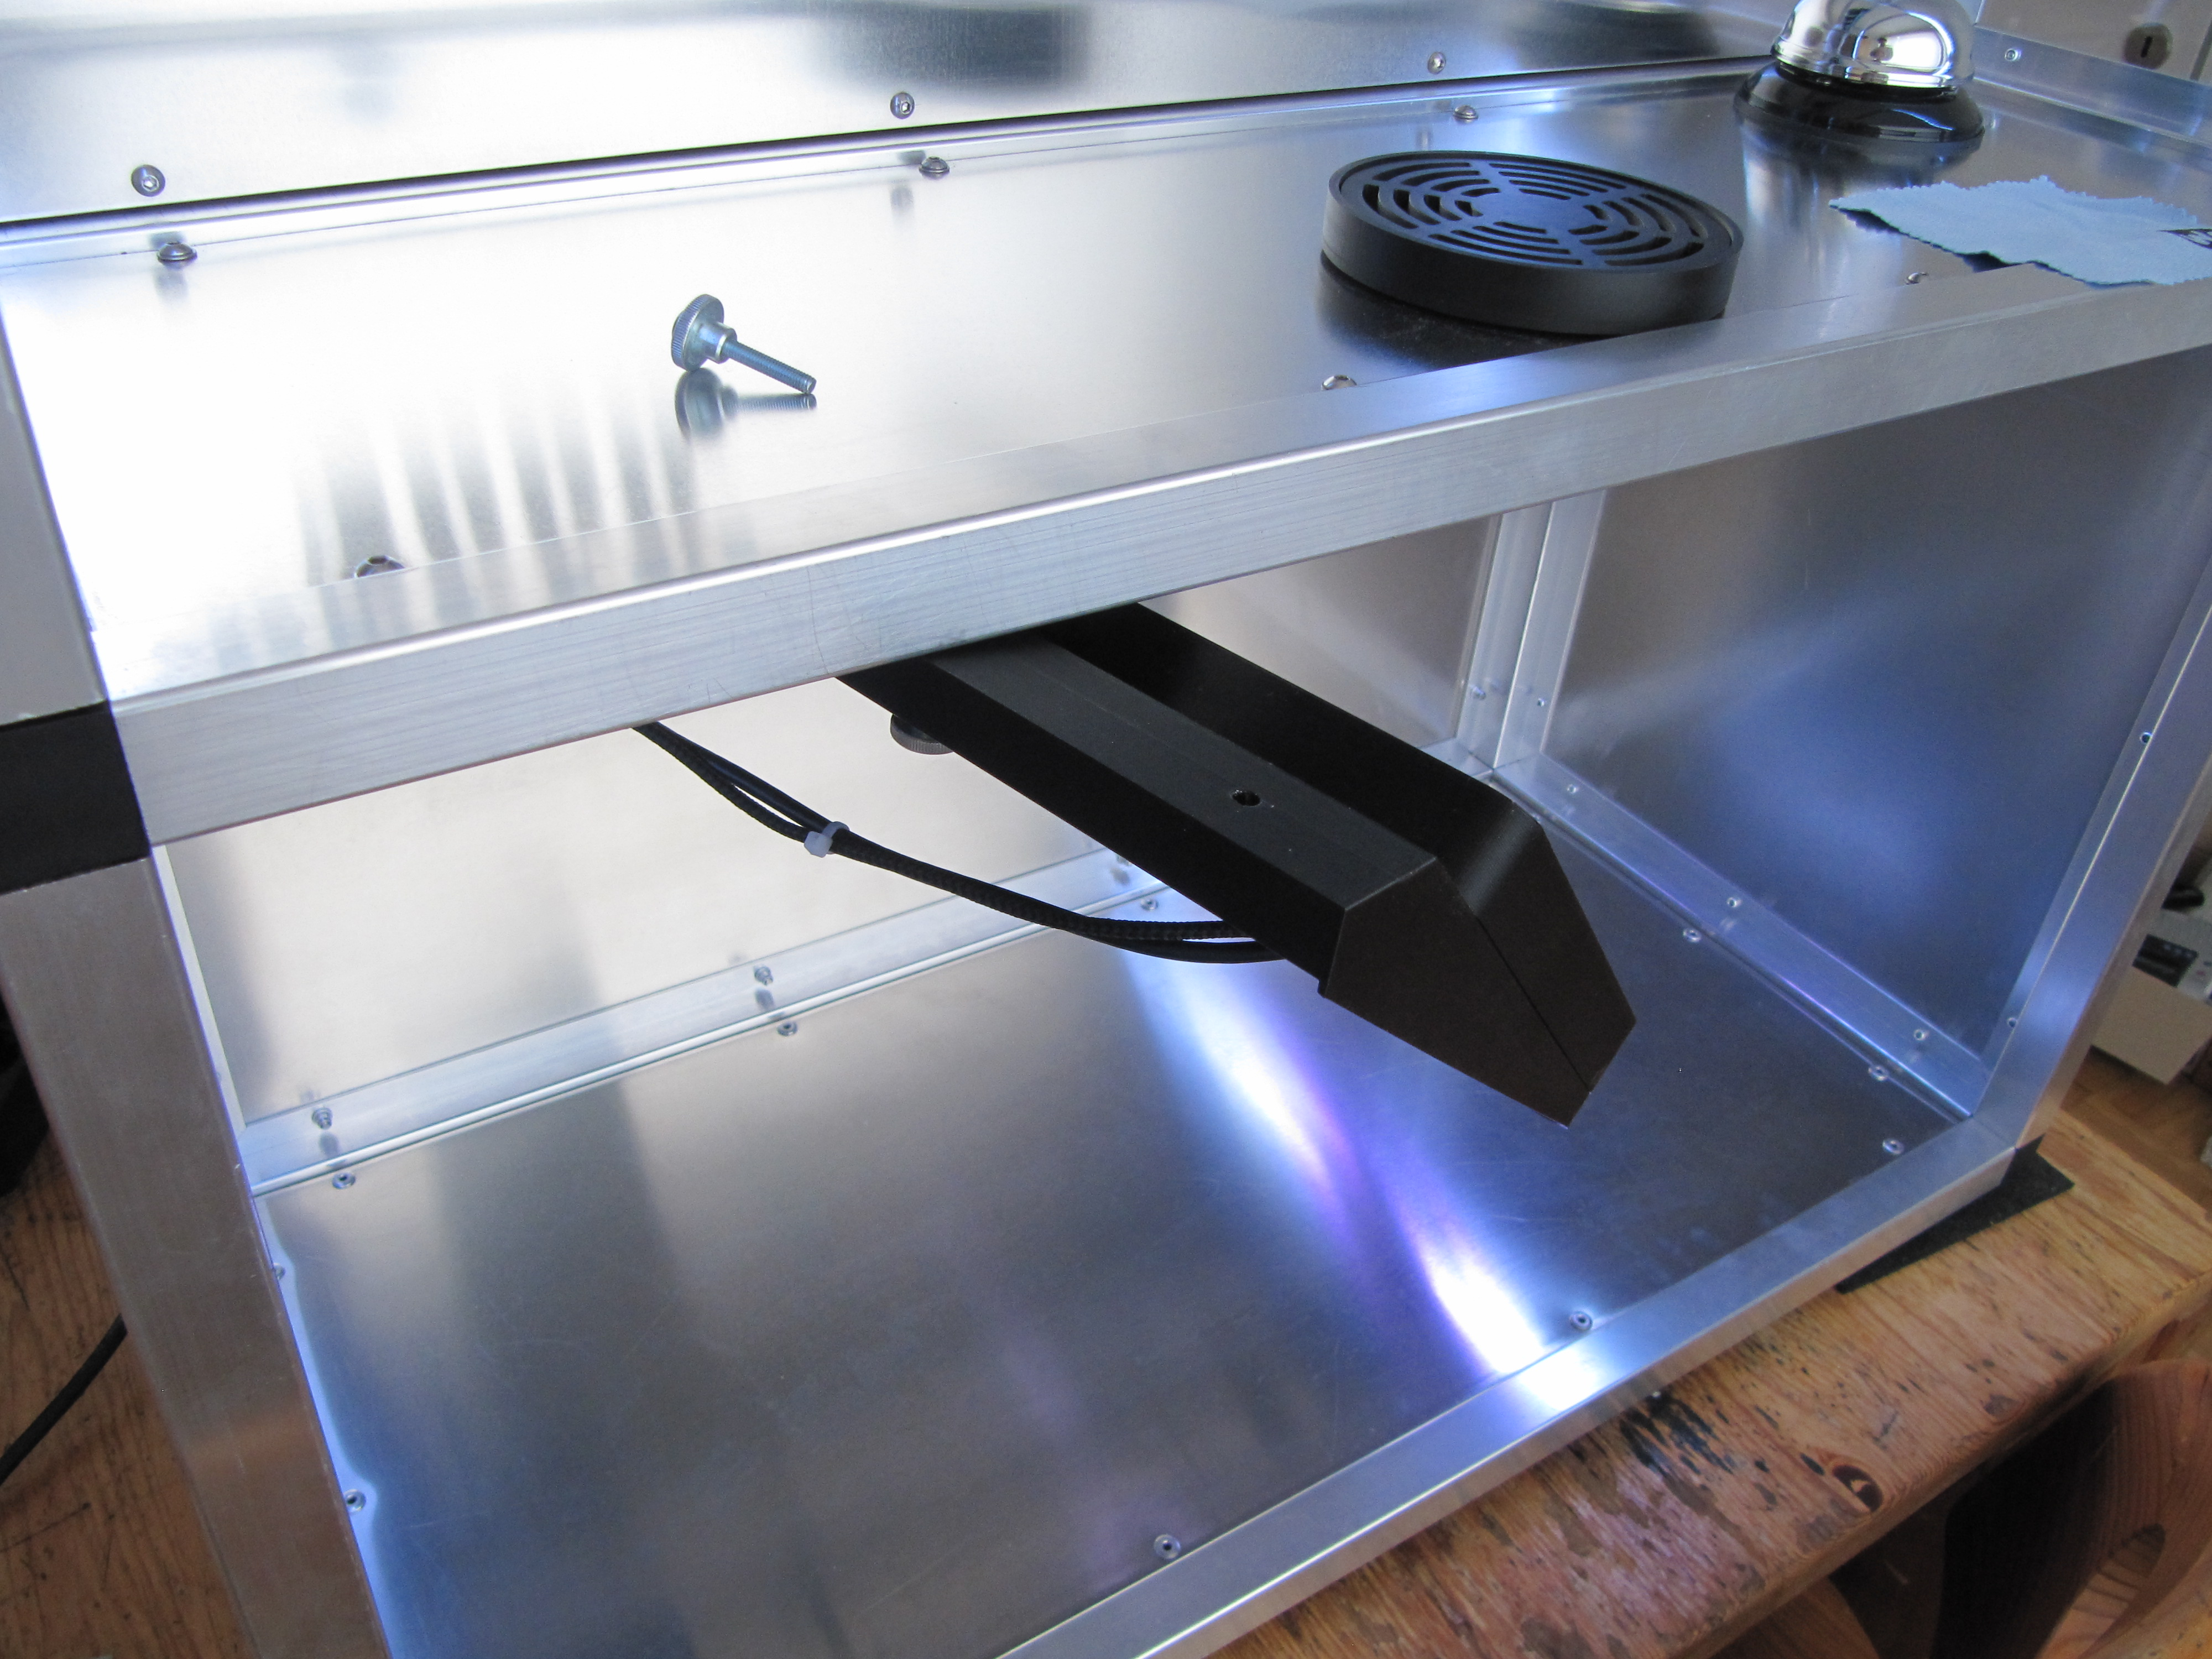
\includegraphics[height=8cm]{pics/Display_half.jpg}}
 \subfigure[Display flipped]{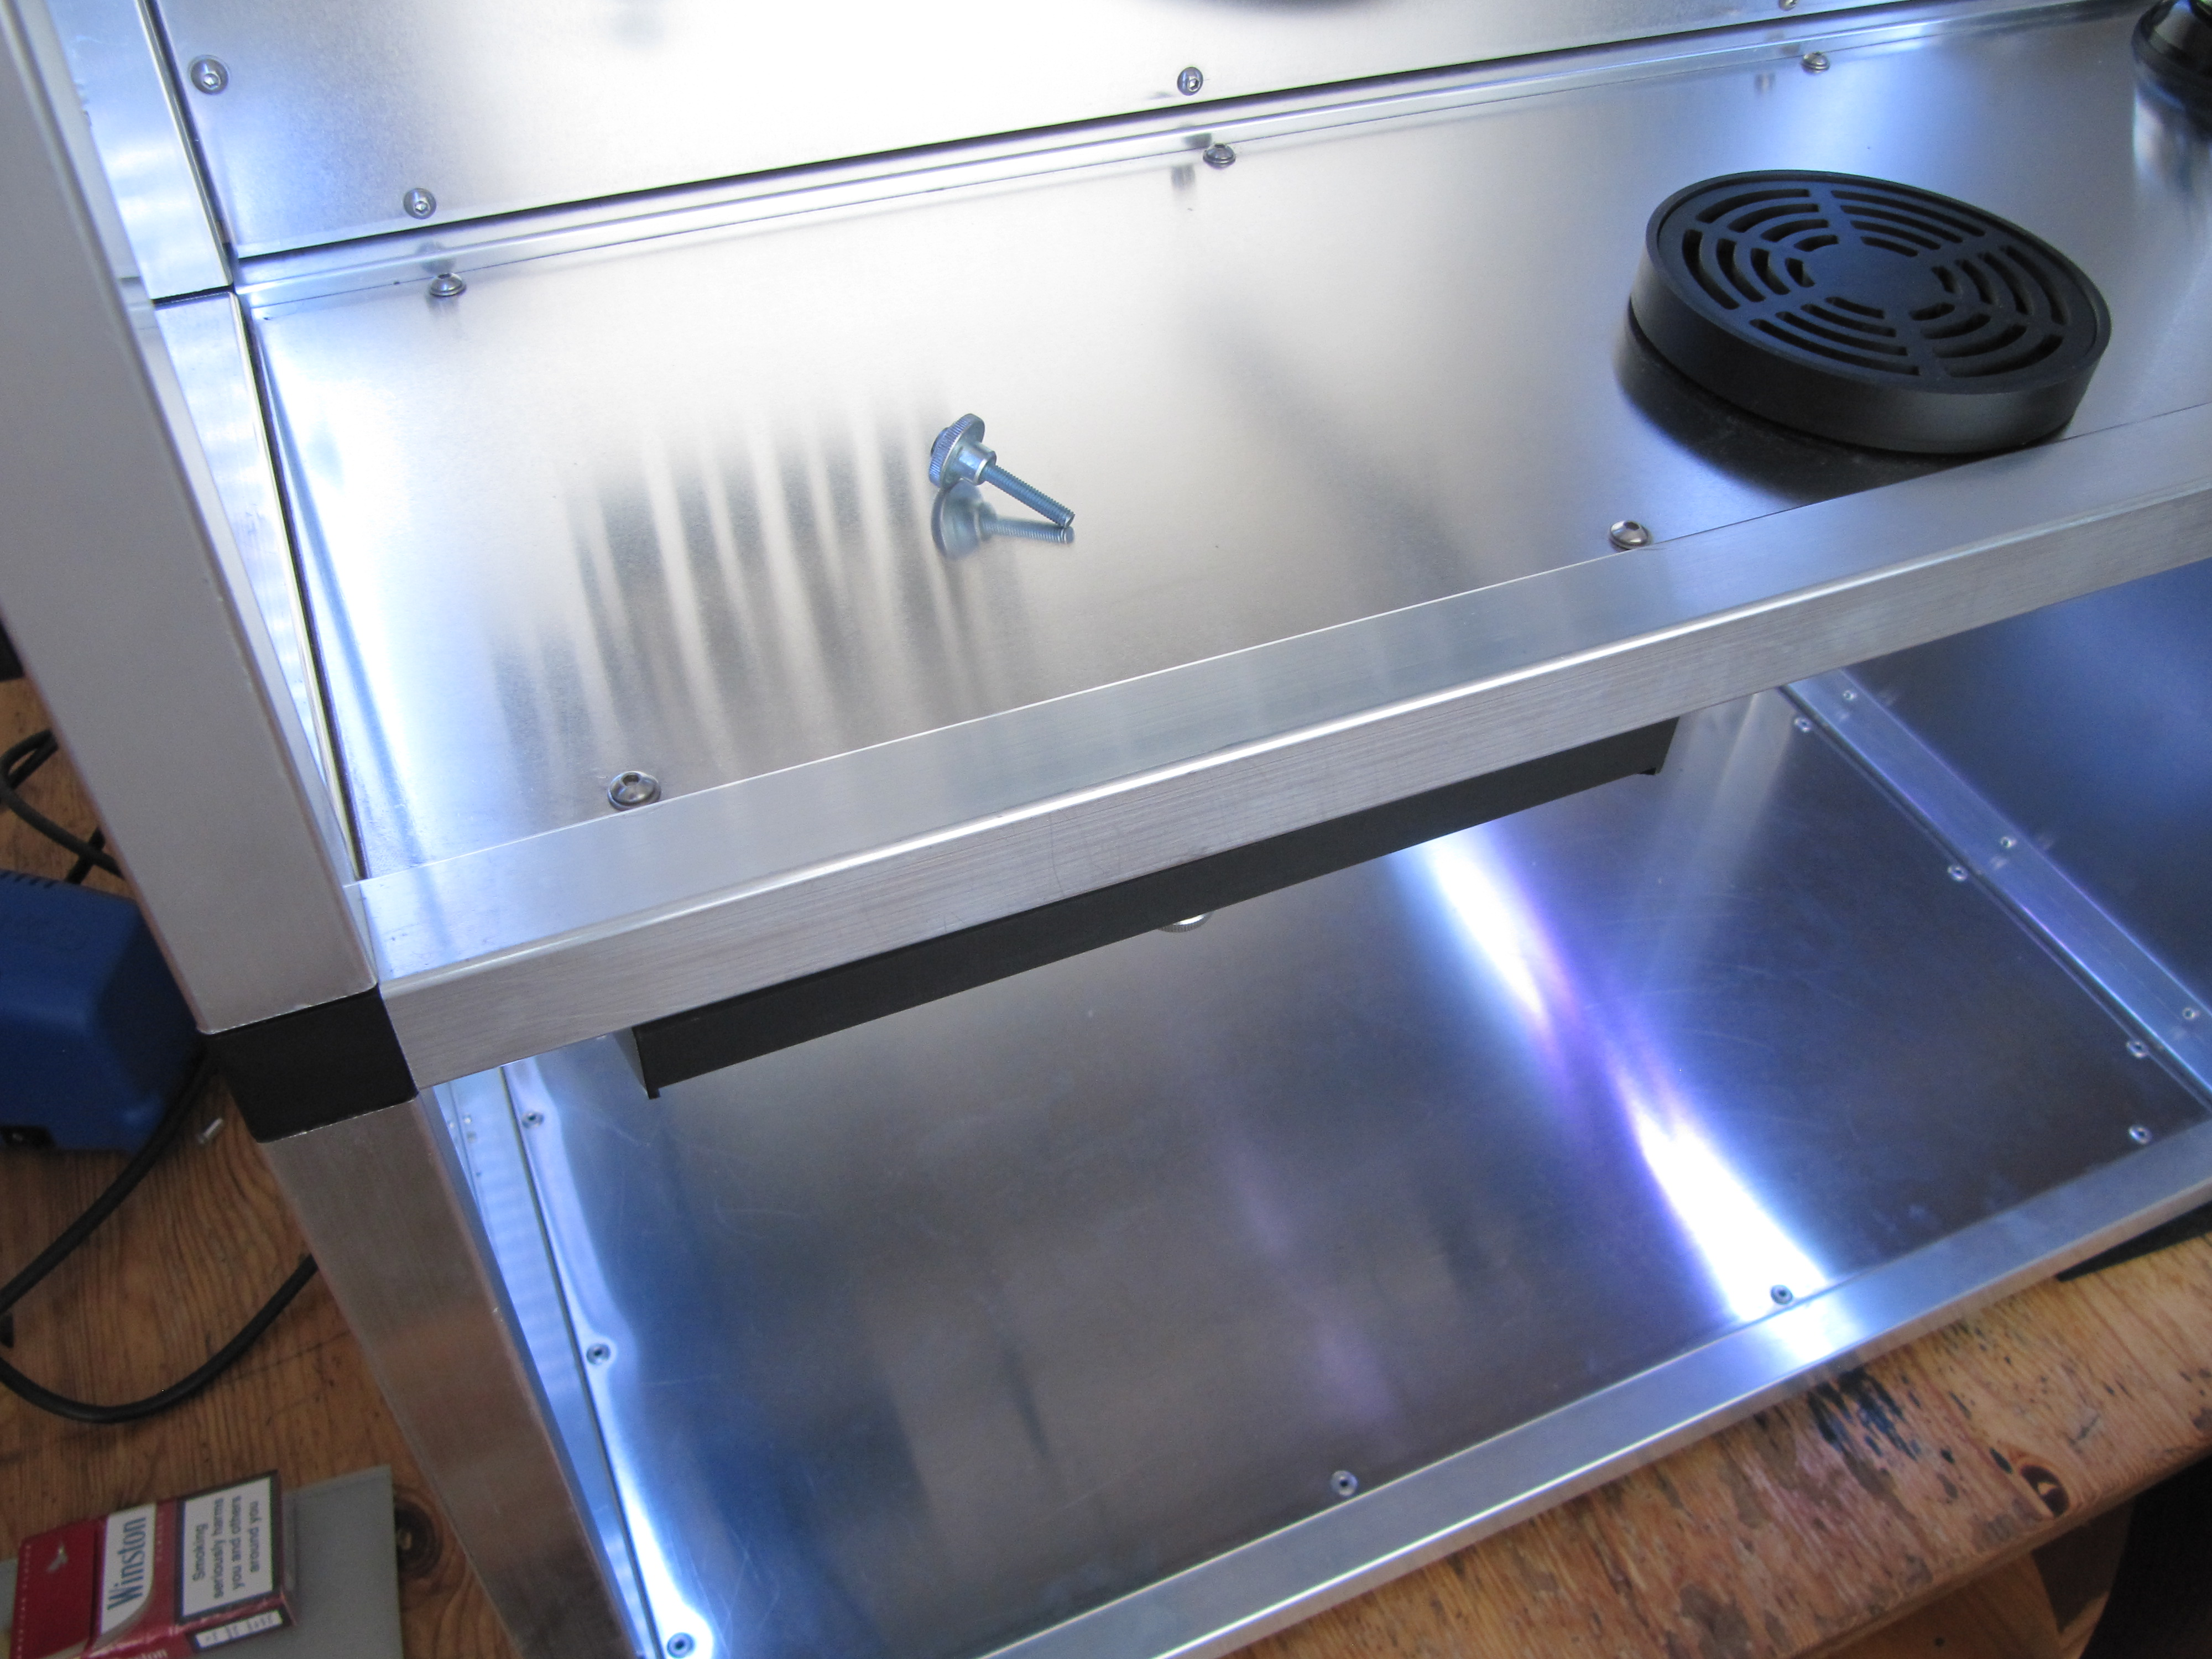
\includegraphics[height=8cm]{pics/Display_in.jpg}}
 \caption{Flipped display} \label{display_half_in}
\end{figure}

\subsection{Electronics}

\subsubsection{General}
We decided to realize the power supply of Hector 9000 with a PC power supply. It is recommended to place the voltage outputs of the power supply unit on terminal blocks and to carry out the cable routing in wiring channels. We have fused the supply voltage of the LED strips, also on terminal blocks. It is also useful to make the connections between the modules by crimped connectors.    

\begin{figure}
  \centering
  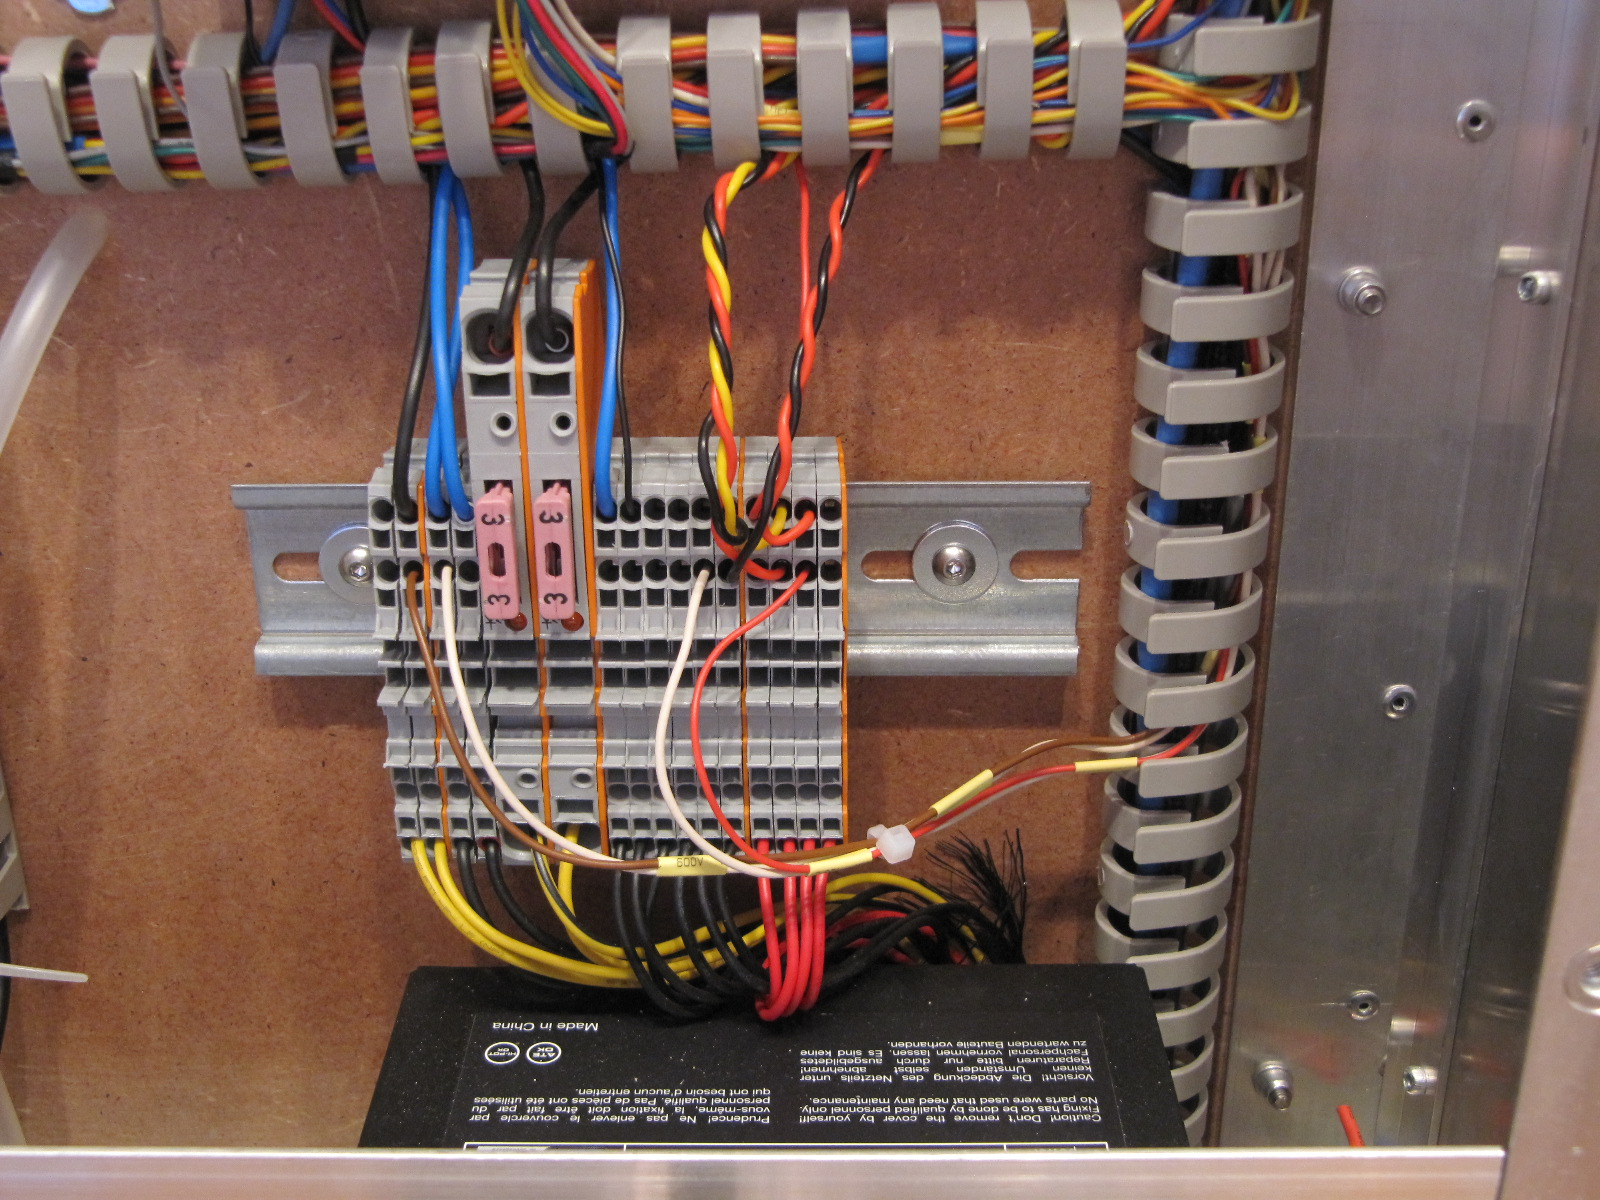
\includegraphics[height=8cm]{pics/psu}
  \caption{Power supply} \label{psu}
\end{figure}

\begin{figure}
  \centering
  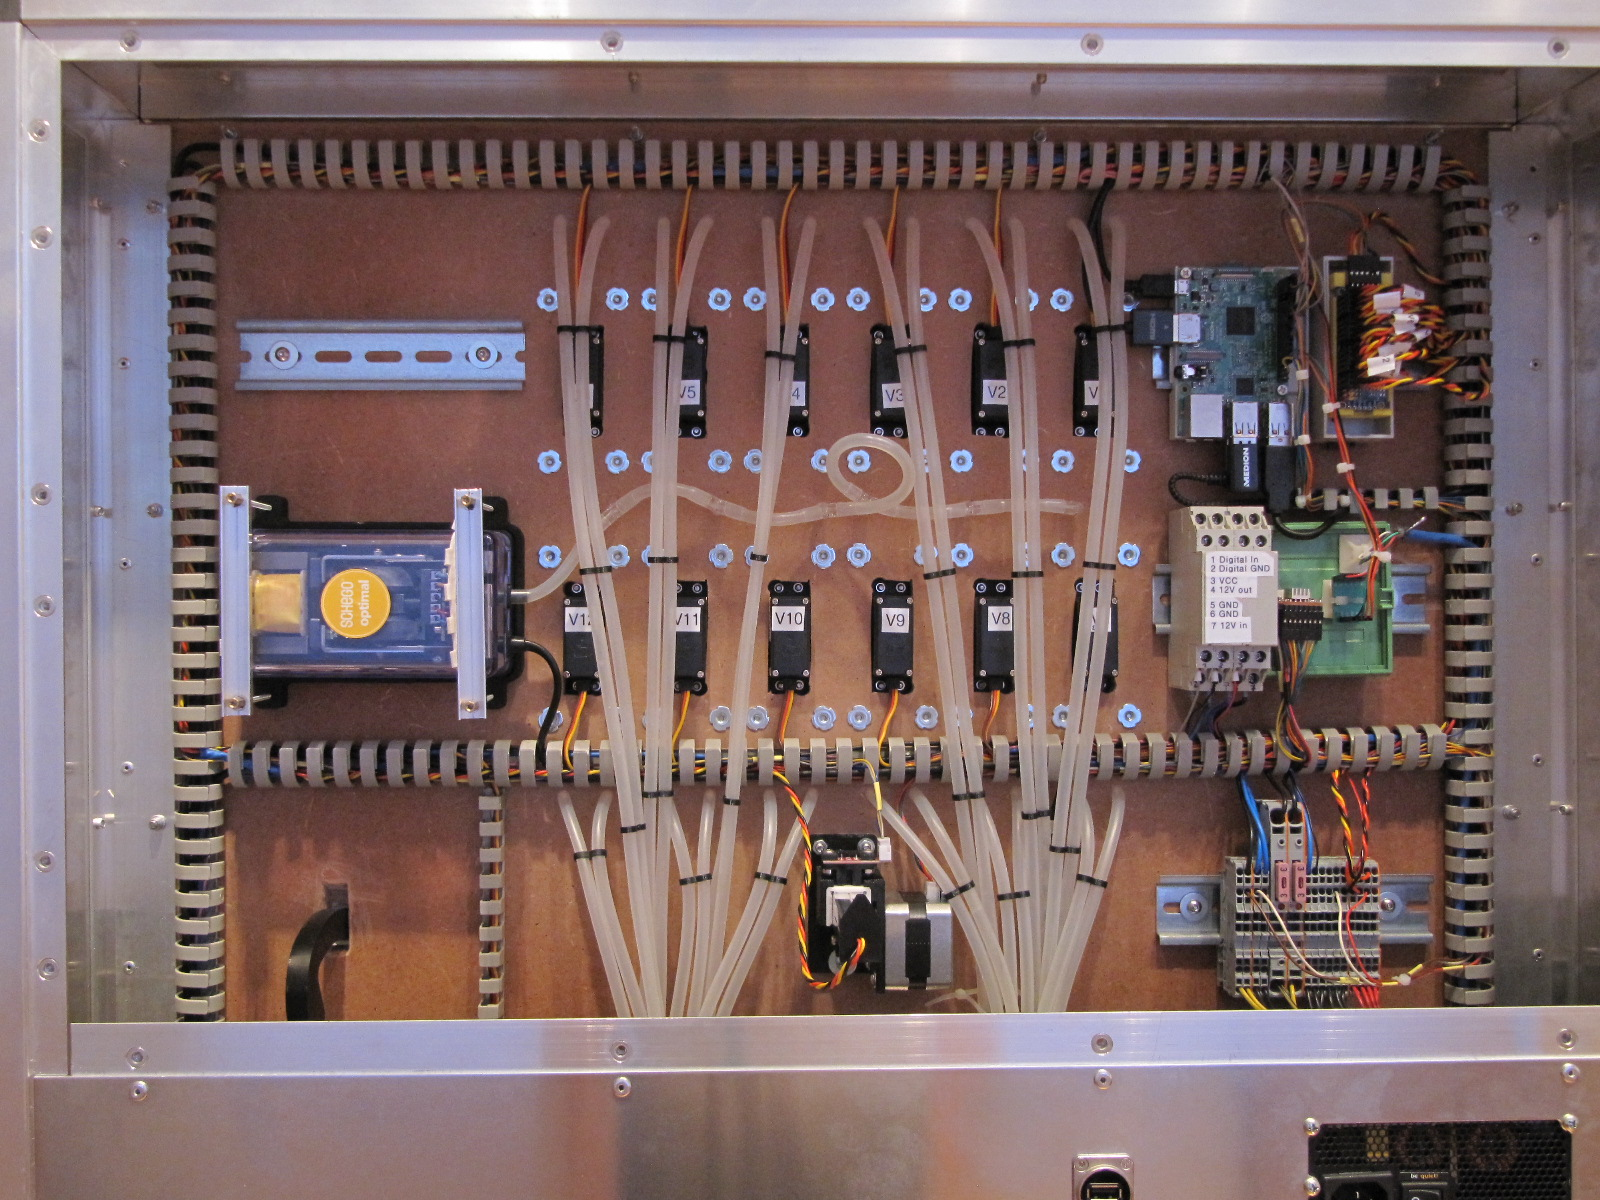
\includegraphics[height=8cm]{pics/electronic_overview}
  \caption{Backpanel removed} \label{electronic_overview}
\end{figure}

\subsubsection{Wiring}
The interconnection of the individual components (Fig.\,\ref{GPIO_overview}) is relatively simple. We recommend placing the HX711 board as close as possible to the Raspberry Pi in order to keep the I2C lines short. For the illumination two WS2812B LED strips were connected in parallel to the GPIO of the RPi. There are 15 LEDs in the lower compartment (bottles) per line and 30 LEDs in the upper compartment of the housing. The pinout of the Raspberry Pi can be seen in Fig.\,\ref{GPIO_connections}. The optional all-round light must be switched via a transistor (Fig.\,\ref{rundumlicht}).  

\begin{figure}
  \centering
  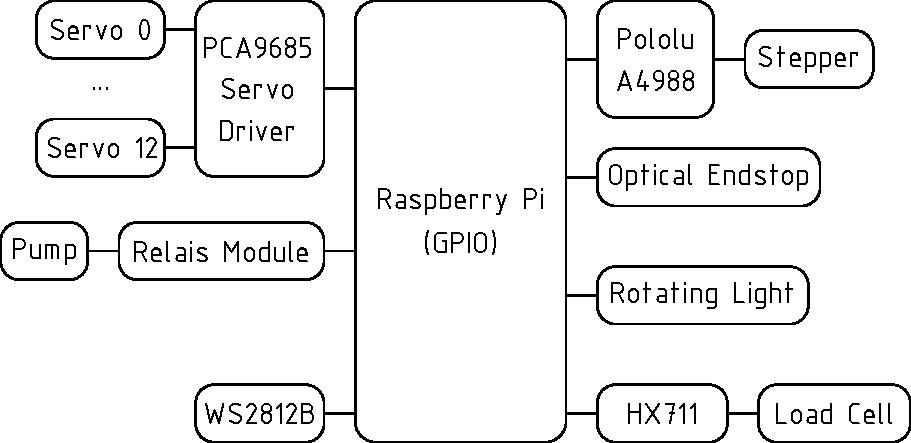
\includegraphics[height=6cm]{pics/RPi_GPIO_overview.pdf}
  \caption{Wiring overview} \label{GPIO_overview}
\end{figure}

\begin{figure}
  \centering
  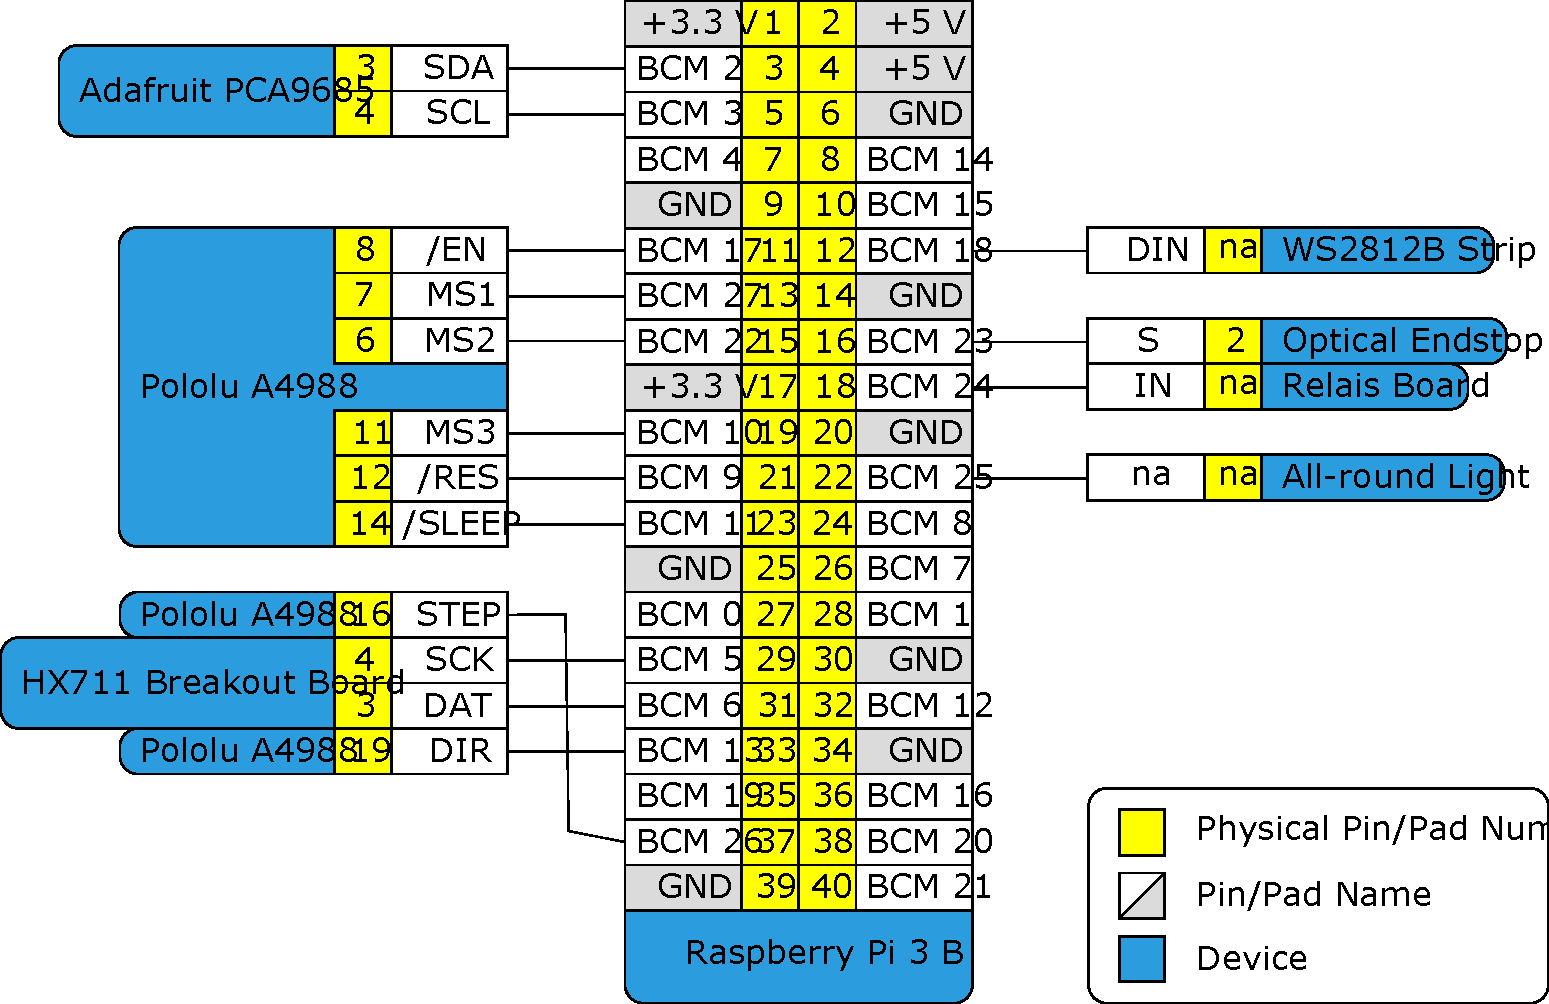
\includegraphics[height=9cm]{pics/Hector9000_connections.pdf}
  \caption{GPIO connections} \label{GPIO_connections}
\end{figure}

\begin{figure}
  \centering
  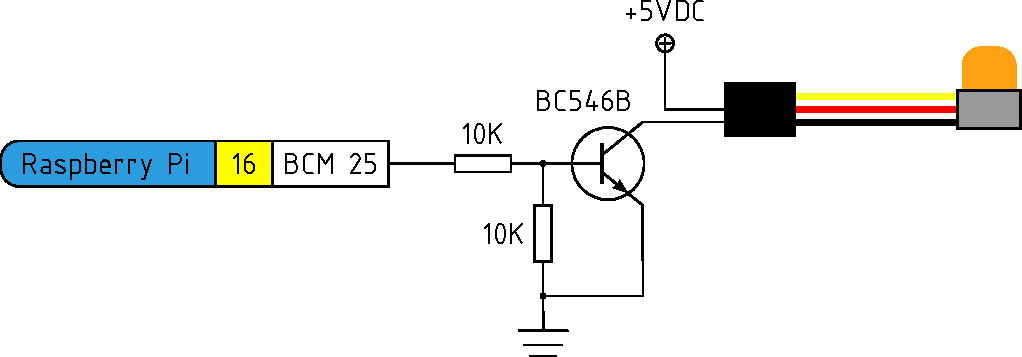
\includegraphics[height=5cm]{pics/rundumlicht.pdf}
  \caption{Connecting the all-round light} \label{rundumlicht}
\end{figure}

\FloatBarrier
\subsection{BOM}
The BOM only lists components that are necessary to manufacture the individual assemblies. \textbf{Cables, plugs, DIN rails, wiring channels, \uline{material for mounting the modules in the housing}, etc. must be put together individually depending on your housing.} In the column \textit{Source} is listed where we got the parts; these sources are not an advertisement or recommendation for certain sellers or platforms, but are merely intended to indicate where the material could be sourced.

\begin{table}
\caption{BOM Scale}
\begin{tabular}{|l|l|l|l|}
\hline
Qty. & Title & Decription & Source\\
\hline\hline
1 & Overflow grid & \texttt{Scale\_overflow\_grid.stl} & 3D printed \\
\hline 
1 & Overflow pipe & \texttt{Scale\_overflow\_pipe.stl} & 3D printed\\
\hline 
1 & Scale pan & \texttt{Scale\_pan.stl} & 3D printed\\
\hline
1 & Spacer & \texttt{Scale\_spacer.stl} & 3D printed\\
\hline
1 & Case & \texttt{Scale\_cover.stl} & 3D printed \\
\hline 
1 & Lid & \texttt{Scale\_lid.stl} & 3D printed\\
\hline 
1 & Cable gland M10&  & eBay\\
\hline 
4 & Screw for thermoplasts 3x10& & Wegertseder\\
\hline
1 & Load cell \SI{1}{\kilo\gram} with HX711 board & &Amazon\\
\hline
\end{tabular}
\end{table}

\begin{table}
\caption{BOM Pump}
\begin{tabular}{|l|l|l|l|}
\hline
Qty. & Title & Description & Source\\
\hline\hline
1 & Mounting base & \texttt{Schego\_830\_mount.stl} & 3D printed \\
\hline
1 & Schego 830 membrane pump & &Amazon\\
\hline 
2 & Foam rubber strips \SI{13}{\milli\metre} x \SI{70}{\milli\metre} & & DIY Store \\
\hline
2 & Aluminium U-profile \SI{13}{\milli\metre} x \SI{8}{\milli\metre} x \SI{105}{\milli\metre} & & DIY Store\\
\hline 
4 & Threaded rod M3x65 & & DIY Store\\
\hline
12 & DIN 934 Nut M3 & & Wegertseder\\
\hline
\end{tabular}
\end{table}

\begin{table}
\caption{BOM Valves}
\begin{tabular}{|l|l|l|l|}
\hline
Qty. & Title & Description & Source\\
\hline\hline
12 & Valve body & \texttt{Valve\_body.stl} & 3D printed \\
\hline 
12 & Cam & \texttt{Valve\_cam.stl} & 3D printed\\
\hline
24 & Tongue & \texttt{Valve\_tongue.stl} & 3D printed\\
\hline
12 & Cover PMMA & \texttt{Valve\_cover.stl} & CNC/Laser \\
\hline 
12 & TowerPro MG996R servo & only genuine & Hobbyking\\
\hline 
24 & DIN 965 Bolt M3x8 & & Wegertseder\\
\hline
48 & ISO 7380 Bolt M3x10 &  & Wegertseder\\
\hline
24 & DIN 933 Bolt M3x35 &  & Wegertseder\\
\hline
72 & DIN 934 Nut M3 & & Wegertseder\\
\hline 
24 & DIN 466 Knurled nut M3 &  & Wegertseder\\
\hline 

\end{tabular}
\end{table}

\begin{table}
\caption{BOM Arm}
\begin{tabular}{|l|l|l|l|}
\hline
Qty. & Title & Description & Source\\
\hline\hline
1 & Mounting bracket & \texttt{Arm\_mount.stl} & 3D printed\\
\hline
1 & Slide insert & \texttt{Arm\_sliding\_element.stl} & 3D printed\\
\hline
1 & Rack & \texttt{Arm\_rack.stl}  & 3D printed\\
\hline
1 & Pinion & \texttt{Arm\_pinion.stl}  & 3D printed\\
\hline
1 & Trigger & \texttt{Arm\_trigger.stl} & 3D printed\\
\hline
1 & Dosing head & \texttt{Arm\_pourer.stl} & 3D printed\\
\hline
1 & Drip catcher & \texttt{Arm\_drip\_pan.stl}  & 3D printed\\
\hline
1 & Optical endstop &  & Amazon\\
\hline 
1 & Pololu A4988 & & Amazon\\
\hline 
1 & NEMA 17 Stepper & & Amazon\\
\hline
1 & Aluminium square tube 15.5x15.5 & Lenght depends on your housing& DIY Store\\
\hline
1& DIN 7981 Self tapping screw 2.9x6.5  & & Wegertseder\\
\hline
4 & ISO 7380 Bolt M3x6  & & Wegertseder\\
\hline
4 & ISO 7380 Bolt M3x10  & & Wegertseder\\
\hline
6 & DIN 125 Washer 3.2  & & Wegertseder\\
\hline
2 & DIN 934 Nut M3 & & Wegertseder\\
\hline
3 & DIN 934 Nut M4 & & Wegertseder\\
\hline
1 & DIN 466 Knurled nut M4 &  & Wegertseder\\
\hline 
6 & DIN 125 Washer 3.2  & & Wegertseder\\
\hline
2 & Blind rivet nut M3x10 flat & & Wegertseder\\
\hline 

\end{tabular}
\end{table}

\begin{table}
\caption{BOM Bell}
\begin{tabular}{|l|l|l|l|}
\hline
Qty. & Title & Description & Source\\
\hline\hline
1 & Bracket for the bell & \texttt{Bell\_base.stl} & 3D printed\\
\hline
1 & Bracket for the motor & \texttt{Bell\_servo-bracket.stl}& 3D printed\\
\hline 
1 & Finger & \texttt{Bell\_finger.stl} & 3D printed\\
\hline
1 & TowerPro MG996R servo & only genuine & HobbyKing\\
\hline
1 & Bell &  & Amazon \\
\hline
7 & ISO 7380 Bolt M3x10  & & Wegertseder\\
\hline
7 & ISO 7380 Bolt M3x12  & & Wegertseder\\
\hline
11 & DIN 934 Nut M3& & Wegertseder\\
\hline 
 
\end{tabular}
\end{table}

\begin{table}
\caption{BOM Plugs}
\begin{tabular}{|l|l|l|l|}
\hline
Qty. & Title & Description & Source\\
\hline\hline
12 & Core for the plugs & \texttt{Rubberplug\_core.stl} & 3D printed\\
\hline
12 & Long-Life Corky \SI{0.7}{\litre}-\SI{1.0}{\litre} &  & METRO\\
\hline 
\end{tabular}
\end{table}

\begin{table}
\caption{BOM Display}
\begin{tabular}{|l|l|l|l|}
\hline
Qty. & Title & Description & Source\\
\hline\hline
1 & Cover & \texttt{Display\_lid.stl} & 3D printed \\
\hline 
1 & Base & \texttt{Display\_base.stl} & 3D printed\\
\hline
1 & Clamp & \texttt{Display\_clamp.stl} & 3D printed\\
\hline
1 & 7'' Touch display & Touch function via USB! & Amazon\\
\hline
4 & Distance bolt M3 x 10 & male-female &Amazon\\
\hline
2 & Screw for thermoplasts 3x10& & Wegertseder\\
\hline
4 & ISO 7380 Bolt M3x16  & & Wegertseder\\
\hline
4 & DIN 934 Nut M3 & & Wegertseder\\
\hline 
\end{tabular}
\end{table}

\begin{table}
\caption{BOM Misc.}
\begin{tabular}{|l|l|l|l|}
\hline
Qty. & Title & Description & Source\\
\hline\hline
1 & Adafruit PCA9685 Servo driver & & Amazon \\
\hline 
1 & Raspberry Pi 3B & & Amazon\\
\hline  
1 & PC-PSU & & Reichelt\\
\hline
ca. \SI{1.5}{\metre} & WS2812B LED Strips & 12\,VDC version! & Amazon\\
\hline
ca. \SI{30}{\metre} & Silicone hose \SI{6}{\milli\metre} x \SI{4}{\milli\metre} & food-safe;                   & Amazon\\
                    &                                                           & do not buy the cheapest one! & \\
\hline 
1 & Flush funnel version A or B & \texttt{Flush-funnel-XY.stl} & 3D printed\\
\hline 
\end{tabular}
\end{table}

\FloatBarrier
\section{Software}
Later versions of this document will contain a description of the software. At the moment you will find information about the software only on https://github.com/H3c702/Hector9000


\section{Licenses}
\subsection{Hardware}
MIT License

\noindent
Copyright (c) 2018 H3c70r

\noindent
Permission is hereby granted, free of charge, to any person obtaining a copy
of the 3D models and associated documentation files (the "{}Models"{}), to deal
in the Models without restriction, including without limitation the rights
to use, copy, modify, merge, publish, distribute, sublicense, and/or sell
copies of the Models, and to permit persons to whom the Models is
furnished to do so, subject to the following conditions:

\noindent
The above copyright notice and this permission notice shall be included in all
copies or substantial portions of the Models.

\noindent
THE MODELS ARE PROVIDED "{}AS IS"{}, WITHOUT WARRANTY OF ANY KIND, EXPRESS OR
IMPLIED, INCLUDING BUT NOT LIMITED TO THE WARRANTIES OF MERCHANTABILITY,
FITNESS FOR A PARTICULAR PURPOSE AND NONINFRINGEMENT. IN NO EVENT SHALL THE
CONSTRUCTORS OR COPYRIGHT HOLDERS BE LIABLE FOR ANY CLAIM, DAMAGES OR OTHER
LIABILITY, WHETHER IN AN ACTION OF CONTRACT, TORT OR OTHERWISE, ARISING FROM,
OUT OF OR IN CONNECTION WITH THE SOFTWARE OR THE USE OR OTHER DEALINGS IN THE
MODELS.

\subsection{Software}
MIT License

\noindent
Copyright (c) 2018 H3c70r

\noindent
Permission is hereby granted, free of charge, to any person obtaining a copy
of this software and associated documentation files (the "{}Software"{}), to deal
in the Software without restriction, including without limitation the rights
to use, copy, modify, merge, publish, distribute, sublicense, and/or sell
copies of the Software, and to permit persons to whom the Software is
furnished to do so, subject to the following conditions:

\noindent
The above copyright notice and this permission notice shall be included in all
copies or substantial portions of the Software.

\noindent
THE SOFTWARE IS PROVIDED "{}AS IS"{}, WITHOUT WARRANTY OF ANY KIND, EXPRESS OR
IMPLIED, INCLUDING BUT NOT LIMITED TO THE WARRANTIES OF MERCHANTABILITY,
FITNESS FOR A PARTICULAR PURPOSE AND NONINFRINGEMENT. IN NO EVENT SHALL THE
AUTHORS OR COPYRIGHT HOLDERS BE LIABLE FOR ANY CLAIM, DAMAGES OR OTHER
LIABILITY, WHETHER IN AN ACTION OF CONTRACT, TORT OR OTHERWISE, ARISING FROM,
OUT OF OR IN CONNECTION WITH THE SOFTWARE OR THE USE OR OTHER DEALINGS IN THE
SOFTWARE.

\bibliography{literatur}

\section{Revisions}

\begin{tabular}{|c|c|l|c|}
\hline
Version & Date & Issue & Editor \\
\hline\hline 
0.1 & 18.06.2018 & Initial version & Cadmium \\
\hline
0.2 & 23.10.2018 & Supplementing content & Cadmium \\
\hline
0.2a & 26.10.2018 & cosmetics \& corrections & kater \\
\hline
\end{tabular}

\newpage



\end{document}
